

In this class, we relax the assumption that
the data points are independently and identically distributed (i.i.d.) 
by moving to a scenario of \emph{structured prediction}, where the inputs are assumed to have
temporal or spacial dependencies. We start by 
considering sequential models, which correspond to a \emph{chain structure}: for instance,
the words in a sentence. In this lecture, we will use part-of-speech
tagging as our example task.  

We start by defining the notation for this lecture in Section~\ref{notation}.
Afterwards, in section~\ref{hmm}, we focus on the well known Hidden Markov Models and in Section~\ref{ml} we describe how to estimate its parameters from labeled data. In Section \ref{decoding} we explain the inference
algorithms (Viterbi and Forward-Backward) for sequence models. These
inference algorithms will be fundamental for the rest of this lecture,
as well as for the next lecture on \emph{discriminative} training of sequence
models. In Section \ref{pos-tagging} we describe the task of 
Part-of-Speech tagging, and how the Hidden Markov Models are suitable for this task. 
Finally, in Section \ref{sec:em} we 
address unsupervised learning of Hidden Markov Models through the Expectation Maximization
algorithm.\todo{NOTA-MA: Falta a ultima Seccao: "`sec:em"'.}

\section*{Today's assignment}

The assignment of today's class is to implement one inference algorithm for Hidden Markov Models, used to find the most likely hidden state sequence given an observation sequence.

\section{Notation}\label{notation}

In what follows, 
we assume a finite set of \emph{observation labels}, 
$\vocab := \{w_1,\ldots,w_J\}$,
and a finite set of \emph{state labels}, 
$\statevocab := \{c_1,\ldots, c_K\}$. We denote by $\vocab^*$, $\statevocab^*$ the two infinite sets of sequences obtained by grouping the elements of each label set including repetitions and the empty string $\varepsilon$\footnotemark\footnotetext{More formally, we say $\vocab^* := \{\varepsilon\} \cup \vocab \cup \vocab^2 \cup \ldots$ and $\statevocab^* := \{\varepsilon\} \cup \statevocab \cup \statevocab^2  \cup \ldots$ is the Kleene closure of each of the two sets above.}. 
Elements of $\vocab^*$ and $\statevocab^*$ 
are \emph{strings of observations} and \emph{strings of states}, 
respectively. 
Throughout this class, we 
assume our input set is $\X = \vocab^*$, 
and our output set is $\Y = \statevocab^*$. 
In other words, 
our inputs are observation sequences, 
$x = x_1 x_2 \ldots x_N$, 
for some $N \in \mathbb{N}$, where each $x_i \in \vocab$;
given such a $x$, we seek 
the corresponding state sequence, 
$y = y_1 y_2 \ldots y_N$, 
where each $y_i \in \statevocab$. We also consider two special states: the ${\tt start}$ symbol,
which starts the sequence, and 
the ${\tt stop}$ symbol, which ends the sequence. 

Moreover, in this lecture we will assume two scenarios:
\begin{enumerate}
\item \emph{Supervised learning.} We will 
train models from a sample set of paired observation and state sequences, $\mathcal{D}_L := \{(x^1,y^1), \ldots, (x^M,y^M)\} \subseteq \X \times \Y$.
\item \emph{Unsupervised learning.} We will
train models from the set of observations only, $\mathcal{D}_U := \{x^1, \ldots, x^M\} \subseteq \X$.
\end{enumerate}
Our notation is summarized in Table~\ref{tab:hmm_notation}.

%Let $\X = \{\sent^1, \ldots, \sent^D\}$ be a training set of independent
%and identically-distributed random variables. In this work $\sent^d$
%(for notation simplicity we will drop the superscript $d$ when
%considering an isolated example) corresponds to a sentence in natural
%language and decomposes as a sequence of observations of length $N$: $\sent = \obs_1 \ldots
%\obs_N$. Each $\obs_n$ is a discrete
%random variable (a \emph{word}),  taking a value $\vv$ from a
%finite vocabulary $\vocab$. Each $\sent$ has an unknown hidden
%structure $\hseq$  that we want to predict. The
%structures are sequences $\hseq = \hs_1 \ldots \hs_N$ of the same
%length $N$ as the observations. Each hidden state $\hs_n$ is a discrete
%random variable and can take a value $\hv$ from a discrete vocabulary $\hvocab$. 
%
%\afm{need to improve notation}

\begin{table}[h]
\begin{center}
\begin{tabular}{|l|l|}
\hline
\multicolumn{2}{|c|}{Notation}\\
\hline
\hline
$\mathcal{D}_L$ & training set (including labeled data)\\
\hline
$\mathcal{D}_U$ & training set (unlabeled data only)\\
\hline
$M$  & number of training examples \\
\hline
$x = x_1 \ldots x_N$  & observation sequence \\
\hline
$y = y_1 \ldots y_N$  & state sequence \\
\hline

$N$  & length of the sequence \\
\hline
$x_i$ &  observation at position $i$ in the sequence, $i \in \{1,\ldots,N\}$\\
\hline
$y_i$ &  state at position $i$ in the sequence, $i \in \{1,\ldots,N\}$\\
%\hline
%${\tt start}, {\tt stop}$ & start and stop symbols\\ conceitos introduzidos na seccao seguinte
\hline
$\vocab$ & observation set\\
\hline 
$J$ & number of distinct observation labels\\
\hline 
$w_j$ & particular observation, $j \in \{1,\ldots,J\}$\\
\hline 
$\statevocab$ & state set\\
\hline 
$K$ & number of distinct state labels\\
\hline 
$c_k$ & particular state, $k \in \{1,\ldots,K\}$\\
\hline  
\end{tabular}
\end{center}
\label{tab:hmm_notation}
\caption{General notation used in this class}
\end{table}








\section{\label{hmm} Hidden Markov Models}

Hidden Markov Models (HMMs) are one of the most common sequence
probabilistic models, and have been applied to a wide variety of
tasks. HMMs are particular instances of directed probabilistic graphical models (or Bayesian networks) which have a chain topology. 
In a
Bayesian network, every random variable is represented as a node in a
graph, and the edges in the graph are directed and represent
probabilistic dependencies between the random variables. For an HMM, the random variables are divided into two sets, the 
\emph{observed variables}, $X = X_1\ldots X_N$, 
and the \emph{hidden variables} $Y = Y_1\ldots Y_N$.
In the HMM
terminology, the observed variables are called \emph{observations}, and the
hidden variables are called \emph{states}. 
The states are generated according to a first order Markov process, in which the $i^{th}$ state $Y_i$ depends only 
of the previous state $Y_{i-1}$. 
Two special states are the ${\tt start}$ symbol,
which starts the sequence, and 
the ${\tt stop}$ symbol, which ends the sequence. 
%Some textbooks describing HMMs omit the stop symbol. 
%While in some applications, one needs not to 
%consider It is useful to artificially introduce a special ``STOP'' state at the end of the sequence, which marks its end. This is useful for two reasons: it sibmplifies the notation, and it also allows our model to cope with sequences of any finite size (otherwise, how would our model cope with natural sentences, which can range from one or two words to dozens?).
%}
In addition, states emit observation symbols. In an HMM, it is assumed that all
observations are independent given the states
that generated them.


As you may find out with today's assignment, 
implementing the inference routines of the HMM can be challenging. We start with a small and very
simple (also very unrealistic!) example. The idea is that you may compute the desired
quantities by hand and check if your implementation yields the correct result. 

\begin{example}

Consider a person who is only interested in four activities: walking in the park ({\tt walk}), shopping ({\tt shop}), cleaning the apartment ({\tt clean}) and playing tennis ({\tt tennis}).
Also, consider that the choice of what the person does on a given day is determined exclusively by the weather on that day, which can be either {\tt rainy} or {\tt sunny}. 
Now, supposing that we observe what the person did on a sequence of days, the question is: 
can we use that information to predict the weather on each of those days? 
To tackle this problem, we assume 
that the weather behaves as a discrete Markov chain: the weather on a
given day depends only on 
the weather on the previous day. 
The entire system can be described as an HMM.

For example, assume we are asked to predict the weather conditions on two different
sequences of days. During these two sequences, we observed the person performing the following activities: 
\begin{itemize}
\item ``{\tt walk walk shop clean}'' 
\item ``{\tt clean walk tennis walk}''
\end{itemize}
This will be our test set.

Moreover, and in order to train our model, we are given access to three different sequences of days, containing both the activities performed by the person and the weather on those days, namely: 
\begin{itemize}
\item ``{\tt walk/rainy walk/sunny shop/sunny clean/sunny}'' 
\item ``{\tt walk/rainy walk/rainy shop/rainy clean/sunny}''
\item ``{\tt walk/sunny shop/sunny shop/sunny clean/sunny}''
\end{itemize}
This will be our training set.

%It is useful to artificially introduce a special ``STOP'' state at the end of the sequence, which marks its end. This is useful for two reasons: it simplifies the notation, and it also allows our model to cope with sequences of any finite size (otherwise, how would our model cope with natural sentences, which can range from one or two words to dozens?).

Figure \ref{hmm} shows the HMM model for the first sequence of the training set, which already includes the {\tt start} and 
{\tt stop} symbols. The notation is summarized in Table \ref{tab:hmm-simple-notation}.
\end{example}
 
\begin{figure}[ht]
\centering
\includegraphics[width=0.7\textwidth]{figs/sequences/hmm_new}
\caption[HMM running example]{\label{fig:hmm}Diagram showing the conditional independence relations of the HMM. As an example, the variables are the values of the first sentence of the training set of the simple sequence.}
\end{figure}

\begin{table}[h]
\begin{center}
\begin{tabular}{|l|l|}
\hline
\multicolumn{2}{|c|}{HMM Notation}\\
\hline
\hline
$x$ & observed sequence ``{\tt walk walk shop clean}'' \\
\hline
$N = 4$ & observation length \\
\hline
$i$ & position in the sentence: $i \in \{1 \ldots N\}$ \\
\hline
$\vocab = \{\text{{\tt walk}},\text{{\tt shop}},\text{{\tt clean}},\text{{\tt tennis}}\}$ & observation set \\
\hline 
$j$ & index into the observation set $j \in \{1,\ldots, J\}$\\
\hline
$X_i = w_j$ & observation at position $i$ 
has value $w_j$\\
\hline 
$\statevocab = \{\text{{\tt rainy}},\text{{\tt sunny}}\}$ & state set\\
\hline 
$k$ & index into state set $k \in \{1,\ldots,K\}$\\
\hline
$Y_i = c_k$ & state at position $i$ has value $c_k$ \\ %acho que nao e necessario baralhar com os parenteses
\hline
\end{tabular}
\end{center}
\caption[HMM notation]{\label{tab:hmm-simple-notation} HMM notation for the simple example.}
\end{table}



\begin{exercise}
Load the simple sequence dataset. 
From the ipython command line create a simple sequence object and look
at the training and test set.
\begin{python}
import lxmls.readers.simple_sequence as ssr
simple = ssr.SimpleSequence()
print simple.train

[walk/rainy walk/sunny shop/sunny clean/sunny , walk/rainy walk/rainy shop/rainy clean/sunny , walk/sunny shop/sunny shop/sunny clean/sunny ]

print simple.test

[walk/rainy walk/sunny shop/sunny clean/sunny , clean/sunny walk/sunny tennis/sunny walk/sunny ]
\end{python}
Get in touch with the classes used to store the sequences, you will need this for the next exercise. Note that each label is internally stored as a number. This number can be used as index of an array to store information regarding that label.
\begin{python}
for sequence in simple.train.seq_list:
    print sequence

walk/rainy walk/sunny shop/sunny clean/sunny
walk/rainy walk/rainy shop/rainy clean/sunny
walk/sunny shop/sunny shop/sunny clean/sunny

for sequence in simple.train.seq_list:
    print sequence.x

[0, 0, 1, 2]
[0, 0, 1, 2]
[0, 1, 1, 2]

for sequence in simple.train.seq_list:
    print sequence.y

[0, 1, 1, 1]
[0, 0, 0, 1]
[1, 1, 1, 1]
\end{python}

\end{exercise}

The probability distributions $P(Y_{i}|Y_{i-1})$ are called \emph{transition probabilities}; the distributions 
$P(Y_{1}|Y_{0} = {\tt start})$ are the \emph{initial probabilities}, and 
$P(Y_{N+1}={\tt stop} |Y_{N})$ the \emph{final probabilities}.%
\footnote{Note that the initial and final probabilities 
are asymmetric.} %
Finally, the distributions $P(X_i|Y_i)$ are called \emph{emission probabilities}. 


A first order HMM model has the following independence assumptions over the joint distribution $P(X=x,Y=y)$:
\begin{itemize}
  \item \textbf{Independence of previous states.} The probability of
    being in a given state at position $i$ only depends on
    the state of the previous position $i-1$. Formally, 
    \begin{equation*}
    P (Y_i = y_i | Y_{i-1} = y_{i-1}, Y_{i-2} = y_{i-2}, \ldots, Y_1 = y_1) = P (Y_i = y_i | Y_{i-1} = y_{i-1})
    \end{equation*} 
    defining a first order Markov chain.%
    \footnote{The order of the Markov chain depends on the number of previous positions taken into account. 
    The remainder of the exposition can be easily extended to higher order HMMs, giving the model more generality, 
    but making inference more expensive.}
  \item \textbf{Homogeneous transition.} The probability of
    making a transition from state $c_l$ to state $c_k$ is independent of
    the particular position in the sequence. That is, for all $i,t \in \{1,\ldots,N\}$,
     \begin{equation*}
    P (Y_i = c_k | Y_{i-1} = c_l) =  P (Y_{t} = c_k | Y_{t-1} = c_l)
     \end{equation*}
    % , so we can simply write //novamente, P_{\mathrm{trans}} so e introduzido depois
     %\begin{equation*}
    %P (Y_i = c_k | Y_{i-1} = c_l) = P_{\mathrm{trans}}(c_k|c_l)
     %\end{equation*}
  \item \textbf{Observation independence.}  The probability of
    observing $X_i = x_i$ at position $i$ is fully determined by the state $Y_i$
    at that position. Formally, 
     \begin{equation*}
     P (X_i = x_i | Y_1=y_1, \ldots, Y_i=y_i, \ldots, Y_N=y_N) = P(X_i = x_i | Y_i = y_i)
      \end{equation*}
      This probability is independent of the
    particular position so, for every $i$ and $t$, we can write:  
     \begin{equation*}
    P(X_i = w_j | Y_i = c_k) = P(X_{t} = w_j | Y_{t} = c_k)
     \end{equation*}
    % = P_{\mathrm{emiss}}(w_j|c_k)$.
\end{itemize}
These conditional independence assumptions are crucial to allow
efficient inference, as it will be described.

%ESTA DEFINIDO LA EM CIMA: We also need to define \emph{initial probabilities}, the probability of starting 
% at each state, and  \emph{final probabilities}, the probability of ending the sequence given that we are at a particular state.
%Furthermore, when dealing with text, it is usual to break the homogeneous transition for the last position, and model the final transitions as independent parameters.

 The distributions that define the HMM model are summarized in Table
\ref{tab:hmm-dist}. 
For each one
of them we will use a short notation to simplify the exposition.
\begin{table}[h]
\begin{center}
\begin{tabular}{|l|l|l|l|}
\hline
\multicolumn{4}{|c|}{HMM distributions}\\
\hline
Name & probability distribution & short notation & array size\\
\hline
\textbf{initial probability} & $P(Y_1 = c_k | Y_0 = \text{\tt start})$ & $P_{\mathrm{init}}(c_k|\text{\tt start})$ & $K$ \\
\hline
\textbf{transition probability} & $P(Y_{i}=c_k|Y_{i-1} = c_l)$ & $P_{\mathrm{trans}}(c_k|c_l)$ & $K\times K$\\
\hline
\textbf{final probability} & $P(Y_{N+1} = \text{\tt stop} | Y_N = c_k)$ & $P_{\mathrm{final}}(\text{\tt stop}|c_k)$ & $K$\\
\hline
\textbf{emission probability} & $P(X_i=w_j| Y_i = c_k)$ & $P_{\mathrm{emiss}}(w_j|c_k)$ & $J \times K$ \\
\hline
\end{tabular}
\end{center}
\caption[HMM probability distributions]{\label{tab:hmm-dist} HMM probability distributions.}
\end{table}

The joint distribution can be expressed as:
\begin{eqnarray}\label{eqn:hmm}
\lefteqn{P(X_1=x_1,\ldots,X_N=x_N,Y_1=y_1,\ldots,Y_N=y_N)=}\nonumber\\
&&
P_{\mathrm{init}}(y_1|\text{\tt start}) 
\times
\left(
\prod_{i=1}^{N-1} P_{\mathrm{trans}}(y_{i+1}|y_i)
\right)
\times
P_{\mathrm{final}}(\text{\tt stop}|y_N)
\times 
\prod_{i=1}^{N} P_{\mathrm{emiss}}(x_i|y_i),
\end{eqnarray}
which for the example of Figure \ref{fig:hmm} is:
\begin{eqnarray}  \label{eqn:hmm_ex}
\lefteqn{P(X_1=x_1,\ldots,X_4=x_4,Y_1=y_1,\ldots,Y_4=y_4)=}\nonumber\\
&&
P_{\mathrm{init}}(\text{\tt rainy}|\text{\tt start}) 
\times
P_{\mathrm{trans}}(\text{\tt sunny}|\text{\tt rainy}) 
\times
P_{\mathrm{trans}}(\text{\tt sunny}|\text{\tt sunny}) 
\times
P_{\mathrm{trans}}(\text{\tt sunny}|\text{\tt sunny}) 
\times\nonumber\\&&
P_{\mathrm{final}}(\text{\tt stop}|\text{\tt sunny}) 
\times
P_{\mathrm{emiss}}(\text{\tt walk}|\text{\tt rainy}) 
\times
P_{\mathrm{emiss}}(\text{\tt walk}|\text{\tt sunny}) 
\times
P_{\mathrm{emiss}}(\text{\tt shop}|\text{\tt sunny}) \nonumber\\&&
\times
P_{\mathrm{emiss}}(\text{\tt clean}|\text{\tt sunny}).
\end{eqnarray}

In the next section we turn our attention to estimating the different
probability distributions of the model.






\section{\label{ml} Finding the Maximum Likelihood Parameters}
%So far we have not committed to any form for the probability
%distributions $\pi_l$, $a_{m,l}$ and $b_l(\obs_i)$. In both applications
%addressed in this class, both the observations and the hidden
%variables are discrete. The most common approach is to model each of
%these probability distributions as multinomial distributions,
%summarized in Table \ref{tt:mult-params}. Note that the number of parameters of $a_{l,m}$ is $|\hvocab|(|\hvocab|+1)$ because of the special ``STOP'' symbol.

%\begin{table}
%\begin{center}
%\begin{tabular}{|c|c|c|c|}
%\hline
%short notation & probability distribution  & |parameters|& constraint \\
%\hline
%$\pi_j$ & $p_{\theta} (\hs_1 = \hv_j)$ & $|\hvocab|$ & $\sum_{\hv \in \hvocab} \pi_j = 1$;\\
%\hline
%$a_{l,m}$ & $p_{\theta} (\hs_i = \hv_l \mid \hs_{i-1} = \hv_m)$ & $|\hvocab|(|\hvocab|+1)$ &$\sum_{\hv_l \in \hvocab} a_{m,l} = 1$;\\
%\hline
%%$f_{l,m}$ & $p_{\theta} (\hs_N = \hv_l \mid \hs_{N-1} = \hv_m)$ & $(|\hvocab|-1)^2$ &$\sum_{\hv_l \in \hvocab} t_{m,l} = 1$;\\
%%\hline
%$b_q(l) $& $p_{\theta}(\obs_i = \vv_q\mid \hs_i = \hv_l)$  & $|\hvocab||\vocab|$ &$\sum_{\vv_q \in \vocab} b_q(l)  = 1$.\\
%\hline
%\end{tabular}
%\end{center}
%\caption[HMM multinomial parametrization]{\label{tt:mult-params}Multinomial parametrization of the HMM distributions.}
%\end{table}

One important problem in HMMs is to estimate the 
model parameters, \emph{i.e.}, 
the distributions depicted in Table~\ref{tab:hmm-dist}. 
We will refer to the set of all these parameters 
as $\theta$. 
In a supervised setting, the HMM model
is trained to maximize the joint log-likelihood of the data. Given a
dataset $\mathcal{D}_L$, the objective being optimized is:
\begin{equation}
\argmax_{\theta} \sum_{m=1}^M \log P_{\theta}(X=x^m,Y=y^m),
\end{equation}
where $P_{\theta}(X=x^m,Y=y^m)$ is given by Eq.~\ref{eqn:hmm}.

In some applications (\emph{e.g.} speech recognition) 
the observation variables are continuous, hence the emission distributions are real-valued (\emph{e.g.} mixtures of Gaussians).
In our case, both the state set and the observation set are discrete (and finite), therefore we use
multinomial distributions for the emission and 
transition probabilities. 
Multinomial distributions are attractive for several reasons: first of
all, they are easy to implement; secondly, the maximum likelihood estimation of the parameters has a simple closed form. The parameters are just
normalized counts of events that occur in the corpus (the same as the
Na\"{i}ve Bayes from previous class).

Given our labeled corpus $\mathcal{D}_L$, the estimation process consists of counting how
many times each event occurs in the corpus and normalize the counts to
form proper probability distributions. Let us define the following
quantities, called sufficient statistics, that represent the counts of
each event in the corpus:

\begin{align}
\mathbf{Initial \ Counts\!:}\;\;\;\;  &  C_{\mathrm{init}}(c_k) = \sum_{m=1}^M
\Ind (y^m_1 = c_k); \label{eq::initialCounts}\\
%
%\mathbf{Final \ Counts\!:}\;\;\;\;  &  fc(\hv_l,\hv _m) = \sum_{\trex} 
%\Ind (\hs_N = \hv_l \mid \hs_{N-1} = \hv_m); \label{eq::finalCounts}\\
%
\mathbf{Transition \ Counts\!:}\;\;\;\;  &  C_{\mathrm{trans}}(c_k,c_l) =
\sum_{m=1}^M  \sum_{i = 2}^{N}
\Ind (y^m_i = c_k \wedge y^m_{i-1} = c_l); \label{eq::transitionCounts}\\
%
\mathbf{Final \ Counts\!:}\;\;\;\;  &  C_{\mathrm{final}}(c_k) = \sum_{m=1}^M
\Ind (y^m_N = c_k); \label{eq::finalCounts}\\
%
\mathbf{Emission \ Counts\!:}\;\;\;\;  &  
C_{\mathrm{emiss}}(w_j,c_k) = \sum_{m=1}^M
\sum_{i = 1}^{N}
\Ind (x^m_i = w_j \wedge y^m_i = c_k); \label{eq::emissionCounts}
\end{align}
Here $y^m_i$,  the underscript denotes the state index position for a given sequence, and the superscript denotes the sequence index in the dataset, and the same applies for the observations.
Note that $\Ind$ is an indicator function that has the value 1 when the
particular event happens, and zero otherwise. In other words, the previous
equations go through the training corpus and count how
often each event occurs. For example, Eq.~\ref{eq::transitionCounts} counts how many times $c_k$ follows state $c_l$. Therefore, $C_{\mathrm{trans}}(\text{\tt sunny},\text{\tt rainy})$ contains the number of times that a sunny day followed a rainy day.

%
%: e.g. the word ``w'' appears with state
%``s'', or state ``s'' follows another state ``s'', or state ``s''
%begins the sentence.


After computing the counts, one can perform some sanity checks
to make sure the implementation is correct. Summing over all entries
of each count table we should observe the following:

\begin{itemize}
\item \textbf{Initial \ Counts\!:} -- Should sum to the number of
  sentences: $\sum_{k=1}^K C_{\mathrm{init}}(c_k) = M$
%\item \textbf{Final \ Counts\!:} - Should sum to the number of sentences.
\item \textbf{Transition/Final \ Counts\!:} -- Should sum to the number of
  tokens: 
  $\sum_{k,l=1}^K C_{\mathrm{trans}}(c_k,c_l) + \sum_{k=1}^K C_{\mathrm{final}}(c_k) = MN$
%   minus 2 times the number of sentences. Note that there are
%  N-1 edges for each sentence, and the last edge is being accounted by
%  the final transitions. So this leaves us with N-2 edges per sentence,
%  where N is the number of tokens in that sentence.
\item \textbf{Emission \ Counts\!:} -- Should sum to the number of tokens: $\sum_{j=1}^J\sum_{k=1}^K C_{\mathrm{emiss}}(w_j,c_k) = MN$.
\end{itemize}

Using the sufficient statistics (counts) the parameter estimates are: 
\begin{align}
  P_{\mathrm{init}}(c_k | \text{\tt start}) &=  \frac{C_{\mathrm{init}}(c_k)}{\sum_{l=1}^K
    C_{\mathrm{init}}(c_l)}\\
  P_{\mathrm{final}}(\text{\tt stop} | c_l) &=  \frac{C_{\mathrm{final}}(c_l)}{\sum_{k=1}^K
    C_{\mathrm{trans}}(c_k,c_l) + C_{\mathrm{final}}(c_l)}\\
  P_{\mathrm{trans}}(c_k | c_l) &=  \frac{C_{\mathrm{trans}}(c_k,c_l)}{\sum_{p=1}^K
    C_{\mathrm{trans}}(c_p,c_l) + C_{\mathrm{final}}(c_l)}\\
  P_{\mathrm{emiss}}(w_j | c_k) &=  \frac{C_{\mathrm{emiss}}(w_j,c_k)}{\sum_{q=1}^J
    C_{\mathrm{emiss}}(w_q,c_k)}
\end{align}


%\begin{exercise}
%Convince yourself that the sanity checks described above are true.
%Collect the counts from a supervised corpus using method
%\emph{collect\_counts\_from\_corpus} and use the provided function \emph{sanity\_check\_counts} to perform these checks on the counts table. 
%%\begin{python}
%% def sanity_check_counts(self,seq_list):
%%\end{python}
%
%\begin{python}
%>>> import sequences.hmm as hmmc
%>>> hmm = hmmc.HMM(simple.x_dict, simple.y_dict)
%>>> hmm.train_supervised(simple.train)
%>>> hmm.sanity_check_counts(simple.train)
%>>> print "Initial Probabilities:", hmm.initial_probs
%
%>>> print "Transition Probabilities:", hmm.transition_probs
%
%>>> print "Final Probabilities:", print 
%hmm.final_probs
%
%>>> print "Emission Probabilities", print hmm.emission_probs
%
%Initial counts match
%Final counts match
%Transition counts match
%Observations counts match
%\end{python}
%\end{exercise}



\begin{exercise}
The provided function \emph{train\_supervised} from the \emph{hmm.py} file implements the above parameter estimates.
%Implement a function that estimates the maximum likelihood
%estimates for the parameters given the corpus in the class HMM.
%The function header is in the hmm.py file. 
%\begin{python}
%def train_supervised(self,sequence_list):
%\end{python}
Run this function given the simple dataset above and look at the estimated probabilities. Are they correct? You can also check the variables ending in \emph{\_counts} instead of \emph{\_probs} to see the raw counts (for example, typing \emph{hmm.initial\_counts} will show you the raw counts of initial states). How are the counts related to the probabilities?

\begin{python}
import lxmls.sequences.hmm as hmmc
hmm = hmmc.HMM(simple.x_dict, simple.y_dict)
hmm.train_supervised(simple.train)
print "Initial Probabilities:", hmm.initial_probs

[ 0.66666667  0.33333333]

print "Transition Probabilities:", hmm.transition_probs

[[ 0.5    0.   ]
 [ 0.5    0.625]]

print "Final Probabilities:", hmm.final_probs

[ 0.     0.375]

print "Emission Probabilities", hmm.emission_probs

[[ 0.75   0.25 ]
 [ 0.25   0.375]
 [ 0.     0.375]
 [ 0.     0.   ]]
\end{python}
\end{exercise}


%%% Local Variables: 
%%% mode: latex
%%% TeX-master: "../../guide"
%%% End: 




\section{\label{decoding} Decoding a Sequence}
Given the learned parameters and a new
observation sequence $x = x_1\ldots x_N$, we want to find the sequence of hidden states $y^* = y_1^* \ldots y_N^*$ that ``best'' explains it.
 This is called the \emph{decoding} problem. There are several ways to define what we mean by the ``best''
$y^*$, depending on our goal: for instance, we may want to minimize the probability of error
on each hidden
variable $Y_i$, or we may want to find the best assignment
to the sequence $Y_1\ldots Y_N$ as a whole. 
Therefore, finding the best sequence
can be accomplished through different approaches:

\begin{itemize}
\item A first approach, normally called \textbf{posterior decoding} or \textbf{minimum risk decoding}, consists
in picking the highest state posterior for each position $i$ in the sequence:
\begin{equation}
y_i^* = \argmax_{y_i \in \Lambda} P(Y_i=y_i | X_1=x_1,\ldots,X_N =x_N).
\end{equation}
%where $\gamma_i(\hs_i)$ is the posterior probability $P(\hs_i|\sent)$. 
Note, however, that this approach does not guarantee that the sequence $y^*=y_1^* \ldots y_N^*$ will be a
valid sequence of the model. For instance, there might be a transition
between two of the best state posteriors with probability zero. 

\item A second approach, called \textbf{Viterbi decoding}, consists in
picking the best global hidden state sequence: 
\begin{eqnarray}
y^* &=& \argmax_{y = y_1\ldots y_N} P(Y_1=y_1,\ldots, Y_N=y_N | X_1=x_1,\ldots,X_N =x_N)\nonumber\\
&=& \argmax_{y = y_1\ldots y_N} P(Y_1=y_1,\ldots, Y_N=y_N, X_1=x_1,\ldots,X_N =x_N).
\end{eqnarray}
\end{itemize}

Both approaches (which will be explained in Sections~\ref{posterior} and~\ref{viterbi}, respectively) rely on dynamic programming and make use of the
independence assumptions of the HMM model. Moreover, they use an alternative
representation of the HMM called a \emph{trellis}. 

A trellis unfolds all possible states for each position and it makes explicit the independence assumption: each position only
depends on the previous position. Here, each column represents a position in the sequence and each row represents a possible state. Figure \ref{fig:trellis} shows the
trellis for the particular example in Figure \ref{fig:hmm}. 

\begin{figure}[ht]
\centering
\includegraphics[width=0.7\textwidth]{figs/sequences/trellis_new}
\caption[HMM Trellis representation.]{\label{fig:trellis} Trellis
  representation of the HMM in Figure ~\ref{fig:hmm}, for the observation
  sequence ``{\tt walk} {\tt walk} {\tt shop} {\tt clean}'', where each hidden variable can take the values {\tt rainy} or {\tt sunny}.}
\end{figure}




Considering the trellis representation, note that we can include the following information:
\begin{itemize}
\item an \emph{initial probability} to the arrows that depart from the start symbol;
\item a \emph{final probability} to the arrows that reach the stop symbol;
\item a \emph{transition probability} to the remaining arrows; and,
\item an \emph{emission probability} to each circle, which is the probability that the observed symbol is emitted by that particular state.
\end{itemize}

For convenience, we will be working with 
log-probabilities, rather than probabilities.\footnote{This will be motivated further in Section~\ref{sec:logdomain}, where we describe 
how operations can be performed efficiently
in the log-domain.} Therefore, if we associate to each circle and arrow in
the trellis a score that corresponds
to the log-probabilities above, 
and if we define the score of a path
connecting the {\tt start} and  {\tt stop} symbols as
the sum of the scores of the circles and arrows
it traverses, 
then 
the goal of finding the most likely sequence of states (Viterbi decoding) corresponds to 
finding the path with the highest score.




%---since 
%we'll be multiplying a lot of probabilities, 
%we prevent underflowing by working in the log-domain. 

%For the decoding algorithms described in the following sections, 
%it is
%useful to define a re-parametrization of the model in equation \eqref{eqn:hmm}, in terms of
%node potentials $\phi_n(l)$ (associating a number to each box in Figure \ref{fig:trellis})
%and edge potentials $\phi_{n-1,n}(l,m)$ (associating a number to each edge in  Figure
%\ref{fig:trellis}). For our example, this re-parametrization is given by
%%
%\begin{equation}
%  \joint =\phi_1(r)\phi_1(r,s)\phi_2(s)\phi_2(s,s)\phi_3(s)\phi_3(s,s)\phi_4(s).
%  \label{eqn:hmm_ex_treelis}
%\end{equation}
%
%%\begin{equation}
%%  \joint =\phi_1(``w'',r)\phi_1(r,s)\phi_2(``w'',s)\phi_2(s,s)\phi_3(``s'',s)\phi_3(s,s)\phi_4(``c'',s).
%%  \label{eqn:hmm_ex_treelis}
%%\end{equation}
%
%In other words, to do this re-parameterization we need to find expressions for the potential variables, (the $\phi$'s) such that \eqref{eqn:hmm} and \eqref{eqn:hmm_ex_treelis} are equal. The solution is given by
%\begin{equation}
%\phi_{i-1,i}(l,m) = a_{l,m}
%\label{eq:nodes1}
%\end{equation}
%and
%\begin{equation}
%\phi_i(l) = 
%\begin{cases}
% b_{\obs_i}(l)\pi_l \quad\text{i = 1}\\
% b_{\obs_i}(l) \quad\text{i = 2,\ldots,N-1}\\
% b_{\obs_i}(l)a_{l,STOP} \quad\text{i = N}
% \label{eq:nodes2}
%\end{cases}
%\end{equation}


%\begin{itemize}
%\item\emph{Edge Potentials} - correspond to the transition parameters, with the exception of the
%edges into the last position that correspond to the final transition parameters.
%\item\emph{Node Potentials} - correspond to the observation
%parameters for a given state and the observation at that position.  The
%first position is the exception and corresponds to the
%product between the observation parameters for that state and
%the observation in that position with the initial parameters for that state. 
%\end{itemize}

%Although this re-parametrization simplifies the exposition, and will be
%used in these lectures, it is not necessarily very practical since we
%will be reproducing several values (for instance the transition
%parameters for each position).


The trellis scores are given by the following expressions:
\begin{itemize}
\item For each state $c_k$:
\begin{eqnarray}
\mathrm{score}_{\mathrm{init}}(c_k) &=&
\log P_{\mathrm{init}}(Y_{1} = c_k | \text{\tt start}).
\end{eqnarray}
\item For each position $i \in {1,\ldots,N-1}$ and each pair of states $c_k$ and $c_l$:
\begin{eqnarray}
\mathrm{score}_{\mathrm{trans}}(i, c_k, c_l) &=&
\log P_{\mathrm{trans}}(Y_{i+1} = c_k | Y_i = c_l).
\end{eqnarray}
\item For each state $c_l$ (\textbf{verify equation: remove $i$ from score?}):
\begin{eqnarray}
\mathrm{score}_{\mathrm{final}}(i, c_l) &=&
\log P_{\mathrm{final}}(\text{\tt stop} | Y_N = c_l).
\end{eqnarray}
\item For each position $i \in {1,\ldots,N}$ and state $c_k$:
\begin{eqnarray}
\mathrm{score}_{\mathrm{emiss}}(i, c_k) &=&
\log P_{\mathrm{emiss}}(X_i = x_i | Y_i = c_k).
\end{eqnarray}
\end{itemize}

In the next exercise, you will compute the trellis scores.

\begin{exercise}
Convince yourself that the score of a path in the trellis 
(summing over the scores above) is equivalent 
to the log-probability $\log P(X=x,Y=y)$, 
as defined in 
Eq.~\ref{eqn:hmm_ex}. 
Use the given function \emph{compute\_scores} on the first training sequence and confirm that the values are correct. You should get the same values as presented below.

%Implement a function that builds the node and edge potentials for a
%given sequence. The function head is in the \emph{hmm.py} file:

%\begin{python}
% def build_potentials(self,sequence):
%\end{python}
%
%Run this function for the first training sequence from the simple
%dataset and compare the results given (If the results are the same
%then you are ready to go).

\begin{python}
>>> initial_scores, transition_scores, final_scores, emission_scores = hmm.compute_scores(simple.train.seq_list[0])
>>> print initial_scores
[-0.40546511 -1.09861229]
>>> print transition_scores
[[[-0.69314718        -inf]
  [-0.69314718 -0.47000363]]

 [[-0.69314718        -inf]
  [-0.69314718 -0.47000363]]

 [[-0.69314718        -inf]
  [-0.69314718 -0.47000363]]]
>>> print final_scores
[       -inf -0.98082925]
>>> print emission_scores
[[-0.28768207 -1.38629436]
 [-0.28768207 -1.38629436]
 [-1.38629436 -0.98082925]
 [       -inf -0.98082925]] 
\end{python}

Note that scores which are $-\infty$ (\texttt{-inf}) correspond
to zero-probability events. 
\end{exercise}

\subsection{Computing in log-domain}\label{sec:logdomain}

We will see that the decoding algorithms 
will need to multiply twice as many probability terms as 
the length $N$ of the sequence. 
This may cause underflowing problems 
when $N$ is large, since the nested multiplication of numbers smaller than 1
may easily become smaller than the machine precision. To avoid that
problem, \cite{rabiner} presents a scaled version of the decoding algorithms that avoids this problem.
An alternative, which is widely used, is computing
in the log-domain. That is, instead of 
manipulating probabilities, manipulate log-probabilities (the scores presented above). 
Every time we need to multiply probabilities, 
we can sum their log-representations, since:
\begin{equation}
\log(\exp(a) \times \exp(b)) = a+b.
\end{equation}
Sometimes, we need to \emph{add} probabilities. 
In the log domain, this requires us to compute 
\begin{equation}
\log(\exp(a) + \exp(b)) = a + \log(1 + \exp(b-a)),
\end{equation}
where we assume that $a$ is smaller than $b$.


\begin{exercise}
Look at the module {\tt sequences/log\_domain.py}. 
This module implements a function
{\tt logsum\_pair(logx, logy)} to 
add two numbers represented in the log-domain;
it returns their sum also represented in the log-domain. The function {\tt logsum(logv)} 
sums all components of an array 
represented in the log-domain. 
This will be used later in our decoding algorithms.
To observe why this is important, type the 
following:
\begin{python}
>>> import numpy as np
>>> a = np.random.rand(10)
>>> np.log(sum(np.exp(a)))
2.8397172643228661
>>> np.log(sum(np.exp(10*a)))
10.121099917705818
>>> np.log(sum(np.exp(100*a)))
93.159220940569128
>>> np.log(sum(np.exp(1000*a)))
inf
>>> from sequences.log_domain import *
>>> logsum(a)
2.8397172643228665
>>> logsum(10*a)
10.121099917705818
>>> logsum(100*a)
93.159220940569114
>>> logsum(1000*a)
925.88496219586864
\end{python}
\end{exercise}


\subsection{Posterior Decoding}\label{posterior}
Posterior decoding consists
in picking state with the highest posterior for each position in the sequence independently; for 
each $i = 1,\ldots,N$:
\begin{equation}
y_i^* = \argmax_{y_i \in \statevocab} P(Y_i=y_i | X = x).
\end{equation}
The \textbf{sequence posterior distribution} is the probability of a particular
hidden state sequence given that we have observed a particular
sequence. Moreover, we will be interested in two other posteriors distributions:
the \textbf{state posterior distribution}, corresponding to the
probability of being in a given state in a certain position given the
observed sequence; and the \textbf{transition posterior distribution},
which is the probability of making a particular transition, from position $i$ to
$i+1$, given the observed sequence. They are formally defined as follows:
\begin{align}
  \mathbf{Sequence \ Posterior\!:}\;\;\;\; &P(Y=y|X=x) = \frac{P(X=x,Y=y)}{P(X=x)}; \label{eq::posteriorDistribution} \\
 \mathbf{State \ Posterior\!:}\;\;\;\;  & P(Y_i=y_i | X=x); \label{eq::nodePosterior} \\
 \mathbf{Transition \ Posterior\!:}\;\;\;\;  &P(Y_{i+1}=y_{i+1},Y_i=y_i| X=x).\label{eq::edgePosterior}
\end{align}

To compute the posteriors, a first step is to be able to compute the 
likelihood of
the sequence $P(X=x)$, which corresponds to summing the probability of all
possible hidden state sequences.
\begin{equation}
\label{likelihoood}
\mathbf{Likelihood\!:}\;\;\;\; P(X=x) = \displaystyle \sum_{y \in \statevocab^N} P(X=x,Y=y).
\end{equation}
The number of possible hidden state sequences is exponential in the
length of the sequence ($|\statevocab|^N$),
 which makes the sum over all of them hard. 
 In our simple
 example, there are $2^4 = 16$ paths, which we can actually explicitly enumerate
 and calculate their probability using Equation \ref{eqn:hmm}. But this is as far as it goes: for example, for Part-of-Speech
 tagging with a small tagset of 12 tags and a medium size
 sentence of length 10, there are $12^{10} = 61 917 364 224$ such
 paths. 
Yet, we must be able to compute this sum (sum over $y \in \statevocab^N$) to compute the above likelihood
formula; this is called the inference problem. For sequence models, there is a well known dynamic programming algorithm,
the \textbf{Forward-Backward} (FB) algorithm, which allows the computation
to be performed in linear time,%
\footnote{The runtime is linear with respect
to the sequence length. More precisely, 
the runtime is $O(N|\statevocab|^2)$. 
A naive enumeration would cost $O(|\statevocab|^N)$.} %
by making use of the independence assumptions.

The FB algorithm relies on the independence of previous states
assumption, which  
is illustrated in the trellis view by having arrows only between consecutive states. 
The FB algorithm defines two auxiliary probabilities, the forward probability and the backward probability. 
\begin{equation}
\label{eq::forward}
\mathbf{Forward \ Probability\!:}\;\;\;\;  \mathrm{forward}(i, c_k) = P(Y_i = c_k, X_1=x_1,\ldots, X_i = x_i)
\end{equation}
The forward probability represents the probability that in position
$i$ we are in state $Y_i = c_k$ and that we have observed $x_1,\ldots,x_i$
up to that position. The forward probability is defined by the
following recurrence rule: 
\begin{eqnarray}
\mathrm{forward}(1, c_k) &=& P_{\mathrm{init}}(c_k|\text{\tt start}) \times 
P_{\mathrm{emiss}}(x_1 | c_k)
 \\
 \mathrm{forward}(i, c_k) &=& \left( \displaystyle \sum_{c_l \in \statevocab} P_{\mathrm{trans}}(c_k | c_l) \times \mathrm{forward}(i-1, c_l) \right) \times P_{\mathrm{emiss}}(x_i | c_k)  \label{forwardRecursion}
 \\
  \mathrm{forward}(N+1, \text{\tt stop}) &=& \sum_{c_l \in \statevocab} P_{\mathrm{final}}(\text{\tt stop} | c_l) \times \mathrm{forward}(N, c_l).
\end{eqnarray}

%\begin{figure}
%\begin{center}
%\begin{tabular}{cc}
%
%\includegraphics[scale=.5]{figs/sequences/forward1}
%& \includegraphics[scale=.5]{figs/sequences/forward2}\\
%\end{tabular}
%\caption[Forward-backward example.]{\label{fig:fb} Forward trellis for
%  the first sentence of the training data at position 1 (left) and at
%  position 2 (right)}
%
%\end{center}
%\end{figure}

%At position 1, the probability of being in state ``r'' and observing word ``w'' is just the node
%marginal for that position: $\alpha_1(r) = \phi_1(r)$ (see Figure
% \ref{fig:fb} left). At position 2 the probability
%of being in state ``s'' and observing the sequence of words ``w w''
%corresponds to the sum of all possible ways of reaching position 2 in
%state ``s'', namely, ``rs'' and ``ss'' (see Figure \ref{fig:fb} right). The probability of the former is
%$\phi_1(r)\phi_1(r,s)\phi_2(s)$
%and that of the latter is $\phi_1(s)\phi_1(s,s)\phi_2(s)$, so we get:
%\begin{eqnarray*}
%   \alpha_2(s) &=& \phi_1(r)\phi_1(r,s)\phi_2(s) +
%   \phi_1(s)\phi_1(s,s)\phi_2(s) \\
%   \alpha_2(s) &=& \left[\phi_1(r)\phi_1(r,s) +
%   \phi_1(s)\phi_1(s,s) \right]\phi_2(s) \\
% \alpha_2(s) &=& \displaystyle \sum_{\hs \in \hvocab}
% \left[\phi_1(\hs)\phi_1(\hs,s)\phi_2(s) \right] \\
%  \alpha_2(s) &=& \displaystyle \sum_{\hs \in \hvocab}
% \left[\alpha_1(\hs)\phi_1(\hs,s)\phi_2(s) \right]
%\end{eqnarray*}

Using the forward trellis one can compute the likelihood simply as:
\begin{equation}
\label{eq:forwardSum}
P(X=x) = \mathrm{forward}(N+1, \text{\tt stop}).
\end{equation}

Although the forward probability is enough to calculate the likelihood
of a given sequence, we will also need the backward probability to
calculate the state posteriors. 
The backward probability is similar to the forward probability, but operates in the inverse direction.
It 
represents the probability of observing $x_{i+1},\ldots,x_N$ from position $i+1$ up to $N$, given that at position $i$ we are at state $Y_i = c_l$:
 \begin{equation}
\label{eq::backward}
\mathbf{Backward \ Probability\!:}\;\;\;\;  \mathrm{backward}(i, c_l) = P(X_{i+1}=x_{i+1},\ldots, X_N=x_N | Y_i = c_l).
\end{equation}
The backward recurrence is given by:
\begin{eqnarray}
\mathrm{backward}(N, c_l) &=& P_{\mathrm{final}}(\text{\tt stop} | c_l) 
 \\
 \mathrm{backward}(i, c_l) &=&  \displaystyle \sum_{c_k \in \statevocab} P_{\mathrm{trans}}(c_k | c_l) \times \mathrm{backward}(i+1, c_k) \times P_{\mathrm{emiss}}(x_{i+1} | c_k)  \label{backwardRecursion}
 \\
  \mathrm{backward}(0, \text{\tt start}) &=& \sum_{c_k \in \statevocab} P_{\mathrm{init}}(c_k | \text{\tt start}) \times \mathrm{backward}(1, c_k) \times P_{\mathrm{emiss}}(x_{1} | c_k).
\end{eqnarray}
%At position $N$ there are no more observations, and the backward
%probability is set to 1. At position $i$, the probability 
%of having observed the future and being in state $\hv_l$, is given by the sum for all possible states of the probability of having transitioned 
%from position $i$ with state $\hv_l$ to position $i+1$ with state $\hv_m$, and observing $\obs_{i+1}$ at time $i+1$ and the future from there onward, which is $\beta_{i+1}(\hs_{i+1} = \hv_m)$. 
Using the backward trellis one can compute the likelihood simply as:.
\begin{equation}
\label{eq:backwardSum}
P(X=x) = \mathrm{backward}(0, \text{\tt start}).
\end{equation}
Moreover, with the forward and backward 
probabilities, we can compute the likelihood of a given sequence using any position $i$ in the sequence
as follows:
\begin{eqnarray}
\label{eq::fbsanity}
  P(X=x) &=& 
  \sum_{c_k \in \statevocab} P(X_1=x_1,\ldots, X_N=x_N,Y_i=c_k)\nonumber\\
  &=&
  \sum_{c_k \in \statevocab} 
  \underbrace{P(X_1=x_1,\ldots, X_i=x_i, Y_i=c_k)}_{\mathrm{forward}(i,c_k)} \times 
  \underbrace{P(X_{i+1}=x_{i+1},\ldots, X_N=x_N| Y_i=c_k)}_{\mathrm{backward}(i,c_k)}\nonumber\\
  &=& \sum_{c_k \in \statevocab} \mathrm{forward}(i,c_k) \times \mathrm{backward}(i,c_k).
\end{eqnarray}

This equation will work for any choice of $i$. Although redundant, this fact is useful when implementing an
HMM as a sanity check that the computations are being performed
correctly, since one can compute this expression for several $i$; they should all yield the same value. 

Algorithm \ref{alg:fb} shows the pseudo code for the forward backward algorithm.



\begin{algorithm}[t]
   \caption{Forward-Backward algorithm \label{alg:fb}}
\begin{algorithmic}[1]
   \STATE {\bfseries input:} sequence $x_1,\ldots,x_N$, scores $P_{\mathrm{init}}, P_{\mathrm{trans}}, P_{\mathrm{final}}, P_{\mathrm{emiss}}$
        \STATE  \emph{Forward pass}: Compute the forward probabilities
        \STATE \emph{Initialization}
        \FOR{$c_k \in \statevocab$ }
        \STATE $\mathrm{forward}(1,c_k) = P_{\mathrm{init}}(c_k|\text{\tt start}) \times 
P_{\mathrm{emiss}}(x_1 | c_k)$
        \ENDFOR 
        \FOR{$i=2$ {\bfseries to} $N$}
         \FOR{$c_k \in \statevocab$ }
                 \STATE $\mathrm{forward}(i, c_k) = \left( \displaystyle \sum_{c_l \in \statevocab} P_{\mathrm{trans}}(c_k | c_l) \times \mathrm{forward}(i-1, c_l) \right) \times P_{\mathrm{emiss}}(x_i | c_k)$
         \ENDFOR 
        \ENDFOR 
       \STATE \emph{Backward pass}: Compute the backward probabilities
       \STATE \emph{Initialization}
        \FOR{$c_l \in \statevocab$ }
        \STATE $\mathrm{backward}(N, c_l) = P_{\mathrm{final}}(\text{\tt stop} | c_l)$
        \ENDFOR 
       \FOR{$i=N-1$ {\bfseries to} 1}
        \STATE $\mathrm{backward}(i, c_l) =  \displaystyle \sum_{c_k \in \statevocab} P_{\mathrm{trans}}(c_k | c_l) \times \mathrm{backward}(i+1, c_k) \times P_{\mathrm{emiss}}(x_{i+1} | c_k)$
        \ENDFOR 
       \STATE \textbf{output:} The forward and backward probabilities.
\end{algorithmic}
\end{algorithm}





\begin{exercise}
%Given the implementation of the forward pass of the forward backward
%algorithm in the file \emph{forward\_backward.py}, implement the backward pass.
%\begin{python}
%
%def forward_backward(node_potentials,edge_potentials):
%    H,N = node_potentials.shape
%    forward = np.zeros([H,N],dtype=float)
%    backward = np.zeros([H,N],dtype=float)
%    forward[:,0] = node_potentials[:,0]
%    ## Forward loop
%    for pos in xrange(1,N):
%        for current_state in xrange(H):
%            for prev_state in xrange(H):
%                forward_v = forward[prev_state,pos-1]
%                trans_v = edge_potentials[prev_state,current_state,pos-1]
%                prob = forward_v*trans_v
%                forward[current_state,pos] += prob
%            forward[current_state,pos] *= node_potentials[current_state,pos]
%    ## Backward loop
%          ## Your code
%   return forward,backward
%
%\end{python}

Run the provided forward-backward algorithm on the first train sequence. 
Observe that both the forward and the backward 
passes give the same log-likelihood.
%Use the provided function that makes use of Equation \ref{eq::fbsanity} to make
%sure your implementation is correct: 
\begin{python}
>>> log_likelihood, forward = hmm.decoder.run_forward(initial_scores, transition_scores, final_scores, emission_scores)
>>> print 'Log-Likelihood =', log_likelihood
Log-Likelihood = -5.06823232601
>>> log_likelihood, backward = hmm.decoder.run_backward(initial_scores, transition_scores, final_scores, emission_scores)
>>> print 'Log-Likelihood =', log_likelihood
Log-Likelihood = -5.06823232601
\end{python}
\end{exercise}


Given the forward and backward probabilities, one can compute both the state
and transition posteriors 
(you can hint why by looking at the term inside the sum in Eq.~\ref{eq::fbsanity}).


\begin{align}
 \mathbf{State \ Posterior\!:}\;\;\;\;  & P(Y_i = y_i| X=x) = \frac{\mathrm{forward}(i, y_i) \times 
 \mathrm{backward}(i, y_i)}{P(X=x)}; \label{eq::nodePosterior2} \\
 \mathbf{Transition \ Posterior\!:}\;\;\;\; &
 P(Y_i = y_i, Y_{i+1} = y_{i+1} | X=x)= \nonumber\\
 &
   \frac{\mathrm{forward}(i, y_i) \times 
   P_{\mathrm{trans}}(y_{i+1}|y_i) \times
   P_{\mathrm{emiss}}(x_{i+1}|y_{i+1}) \times
 \mathrm{backward}(i+1, y_{i+1})}{P(X=x)}.\label{eq::edgePosterior2}
\end{align}

A graphical representation of these posteriors is illustrated in Figure~\ref{fig:posteriors}. 
On the left it is shown that $\mathrm{forward}(i, y_i)  \times \mathrm{backward}(i, y_i)$ returns the sum of all paths that contain the state $y_i$, weighted by $P(X=x)$; on the right we can see that $\mathrm{forward}(i, y_i) \times P_{\mathrm{trans}}(y_{i+1}|y_i) \times P_{\mathrm{emiss}}(x_{i+1}|y_{i+1}) \times \mathrm{backward}(i+1, y_{i+1})$  returns the same for all paths containing the edge from $y_i$ to $y_{i+1}$.
%Thus, these posteriors can be seen as the ratio of the number of paths that contain the given state or transition (weighted by $P(X=x)$) and the number of possible paths in the graph $\marginal$.

As a practical example, given that the person performs the sequence of actions ``{\tt walk} {\tt walk} {\tt shop} {\tt clean}", we want to know the probability of having been raining in the second day. The state posterior probability for this event can be seen as the probability that the sequence of actions above was generated by a sequence of weathers and where it was raining in the second day. In this case, the possible sequences would be all the sequences which have {\tt rainy} in the second position.

\begin{figure}
\begin{center}
\includegraphics[width=1\textwidth]{figs/sequences/posteriors}
\caption[Posterior Illustration.]{\label{fig:posteriors} A graphical representation of the components in the state and transition posteriors. Recall that the observation sequence is ``\texttt{walk walk shop clean}''.}
\end{center}
\end{figure}

%\begin{figure}
%\begin{center}
%\begin{tabular}{cc}
%
%\includegraphics[scale=.5]{figs/sequences/statePost}
%& \includegraphics[scale=.5]{figs/sequences/transPost}\\
%\end{tabular}
%\caption[Posterior Illustration.]{\label{fig:posteriors} A graphical representation of the components in the state and transition posteriors.}
%
%\end{center}
%\end{figure}

Using the state posteriors, we are ready to perform posterior
decoding. 
The strategy is to compute the state posteriors 
for each position $i \in \{1,\ldots,N\}$
and each state $c_k \in \statevocab$, and 
then pick the arg-max at each position:
\begin{equation}
{\widehat y_i} := \argmax_{y_i \in \statevocab} P(Y_i=y_i| X=x).
\end{equation}

%Algorithm \ref{alg:pd} shows the posterior decoding algorithm.

%\begin{algorithm}[t]
%   \caption{Posterior Decoding algorithm \label{alg:pd}}
%\begin{algorithmic}[1]
%   \STATE {\bfseries input:} The forward and backward probabilities
%       $\alpha$ and $\beta$.
%   \STATE  \emph{Compute Likelihood}: Compute the likelihood of the
%   sentence
%   \STATE $L = 0$
%   \FOR{$\hv_l \in \hvocab$ }
%   \STATE $\marginal = \marginal + \alpha_N(\hv_l)$
%   \ENDFOR 
%   \STATE $\hat \hseq = []$
%    \FOR{$i=1$ {\bfseries to} $N$}
%    \STATE $max = 0$
%     \FOR{$\hv_l \in \hvocab$ }
%     \STATE $\gamma_i(\hv_l)  =  \frac{\alpha_i(\hv_l)
%       \beta_i(\hv_l)}{\marginal}$
%     \IF {$\gamma_i(\hv_l) > max$}
%     \STATE $max = \gamma_i(\hv_l)$
%     \STATE $\hat  y_i = \hv_l$
%     \ENDIF
%     \ENDFOR 
%     \ENDFOR 
%   \STATE \textbf{output:} the posterior path $\hat \hseq$
%\end{algorithmic}
%\end{algorithm}



\begin{exercise}
%Given the node and edge posterior formulas \ref{eq::nodePosterior},\ref{eq::edgePosterior} and the
%  forward and backward formulas \ref{eq::forward},\ref{eq::backward}, convince yourself that formulas
%  \ref{eq::nodePosterior2},\ref{eq::edgePosterior2} are correct. 

Compute the node posteriors for the first training sequence (use the provided \emph{compute\_posteriors} function), and look at
the output. Note that the state posteriors are a proper
probability distribution (the lines of the result sum to 1).

\begin{python}
>>> initial_scores, transition_scores, final_scores, emission_scores = hmm.compute_scores(simple.train.seq_list[0])
>>> state_posteriors, _, _ = hmm.compute_posteriors(initial_scores,
                                                    transition_scores,
                                                    final_scores,
                                                    emission_scores)
>>> print state_posteriors
[[ 0.95738152  0.04261848]
 [ 0.75281282  0.24718718]
 [ 0.26184794  0.73815206]
 [ 0.          1.        ]]
\end{python}
\end{exercise}

\begin{exercise}
Run the posterior decode on the first test sequence, and evaluate it.
\begin{python}
>>> y_pred = hmm.posterior_decode(simple.test.seq_list[0])
>>> print "Prediction test 0:", y_pred
walk/rainy walk/rainy shop/sunny clean/sunny
>>> print "Truth test 0:", simple.test.seq_list[0]
walk/rainy walk/sunny shop/sunny clean/sunny 
\end{python}

Do the same for the second test sequence:
\begin{python}
>>> y_pred = hmm.posterior_decode(simple.test.seq_list[1])
>>> print "Prediction test 1:", y_pred
clean/rainy walk/rainy tennis/rainy walk/rainy 
>>> print "Truth test 1:", simple.test.seq_list[1]
clean/sunny walk/sunny tennis/sunny walk/sunny 
\end{python}

What is wrong? Note the observations for the second test sequence: the
observation {\tt tennis} was never seen at training time, so the probability for
it will be zero (no matter what state). This will make all possible state
sequences have zero probability.
As seen in the previous lecture, this is a problem with generative
models, which can be corrected using smoothing (among other
options).

Change the \emph{train\_supervised} method to add smoothing:
\begin{python}
def train_supervised(self,sequence_list, smoothing):
\end{python}

Try, for example, adding 0.1 to all the counts, and repeating this exercise with that smoothing. What do you observe?
\begin{python}
>>> hmm.train_supervised(simple.train, smoothing=0.1)
>>> y_pred = hmm.posterior_decode(simple.test.seq_list[0])
>>> print "Prediction test 0 with smoothing:", y_pred
walk/rainy walk/rainy shop/sunny clean/sunny 
>>> print "Truth test 0:", simple.test.seq_list[0]
walk/rainy walk/sunny shop/sunny clean/sunny
>>> y_pred = hmm.posterior_decode(simple.test.seq_list[1])
>>> print "Prediction test 1 with smoothing:", y_pred
clean/sunny walk/sunny tennis/sunny walk/sunny 
>>> print "Truth test 1:", simple.test.seq_list[1]
clean/sunny walk/sunny tennis/sunny walk/sunny 
\end{python}
\end{exercise}

%Note that if you use smoothing when training, the sanity checks mentioned at the start of this chapter are no longer true. For example, the sum of all the transition counts is no longer equal to the number of tokens -- it is larger.

%\begin{exercise}
%Change the function you just created \emph{ def
%  sanity\_check\_counts(self,seq\_list):} to account for smoothing. Make
%sure it works properly.
%
%\begin{python}
%In []: run sequences/hmm.py
%In []: hmm = HMM(simple)
%In []: hmm.collect_counts_from_corpus(simple.train,smoothing=0.1)
%In []: hmm.sanity_check_counts(simple.train,smoothing=0.1)
%Init Counts match
%Final Counts match
%Transition Counts match
%Observations Counts match
%\end{python}
%\end{exercise}


\subsection{Viterbi Decoding}\label{viterbi}


\textbf{Viterbi decoding} consists in
picking the best global hidden state sequence 
$\widehat{y}$
as follows: 
\begin{equation}
\widehat{y} = \argmax_{y \in \statevocab^N} P(Y=y|X=x) = \argmax_{y \in \statevocab^N} P(X=x,Y=y).
\end{equation}

The Viterbi algorithm 
is very similar to the forward procedure of the FB algorithm,
making use of the same trellis structure to efficiently represent the exponential number of sequences without prohibitive computation costs. In fact, the only
difference from the forward-backward algorithm is in the recursion
\ref{forwardRecursion} where instead of \emph{summing} over all possible 
hidden states, we take their \emph{maximum}.

\begin{equation}
\label{eq::viterbi}
\mathbf{Viterbi }\;\;\;\;  \mathrm{viterbi}(i, y_i) = \max_{y_1...y_{i-1}} P(Y_1=y_1,\ldots Y_i = y_i , X_1=x_1,\ldots, X_i=x_i)
\end{equation}
The Viterbi trellis represents the path with maximum probability in
position
$i$ when we are in state $Y_i=y_i$ and that we have observed $x_1,\ldots,x_i$
up to that position. The Viterbi algorithm is defined by the
following recurrence: 
\begin{eqnarray}
\mathrm{viterbi}(1, c_k) &=& P_{\mathrm{init}}(c_k|\text{\tt start}) \times 
P_{\mathrm{emiss}}(x_1 | c_k)
 \\
 \mathrm{viterbi}(i, c_k) &=& \left( \displaystyle \max_{c_l \in \statevocab} P_{\mathrm{trans}}(c_k | c_l) \times \mathrm{viterbi}(i-1, c_l) \right) \times P_{\mathrm{emiss}}(x_i | c_k)  \label{viterbiRecursion}
 \\
 \mathrm{backtrack}(i, c_k) &=& \left( \displaystyle \argmax_{c_l \in \statevocab} P_{\mathrm{trans}}(c_k | c_l) \times \mathrm{viterbi}(i-1, c_l) \right) \times P_{\mathrm{emiss}}(x_i | c_k) 
 \\
  \mathrm{viterbi}(N+1, \text{\tt stop}) &=& \max_{c_l \in \statevocab} P_{\mathrm{final}}(\text{\tt stop} | c_l) \times \mathrm{viterbi}(N, c_l)
 \\
  \mathrm{backtrack}(N+1, \text{\tt stop}) &=& \argmax_{c_l \in \statevocab} P_{\mathrm{final}}(\text{\tt stop} | c_l) \times \mathrm{viterbi}(N, c_l).
\end{eqnarray}

\todo{\small tirar $\times P_{\mathrm{emiss}}(x_i | c_k)$ no calculo do backtrack? o mesmo no pseudo codigo do algoritmo. ou fazer o argmax de tudo}

%\begin{eqnarray}
%\delta_1(\hv_l) &=& \phi_1(l) \\
%\delta_i(\hv_l) &=& \left[ \max_{y_1 ... y_i} \phi_{i-1,i}(m,l)
%  \delta_{i-1}(\hv_m) \right] \phi_i(l) \label{viterbiRecursion} \\
%\psi_{i}(\hv_l) &=& \left[ \argmax_{y_1 ... y_i} \phi_{i-1,i}(m,l)
%  \delta_{i-1}(\hv_m) \right]
%%\phi_{(i-1)}(m,l)  \delta_{i-1}(\hv_m) \right] \phi_i(l) \label{viterbiBackpointers}
%\end{eqnarray}

Algorithm \ref{alg:viterbi} shows the pseudo code for the Viterbi algorithm.
Note the similarity with the forward algorithm.
The only differences are:
\begin{itemize}
\item Maximizing instead of summing;
\item Keeping the argmax's to backtrack.
\end{itemize}

%\begin{algorithm}[t]
%   \caption{Viterbi algorithm \label{alg:viterbi}}
%\begin{algorithmic}[1]
%   \STATE {\bfseries input:} sentence $\sent$, parameters $\theta$
%        \STATE  \emph{Forward pass}: compute the maximum paths for
%        every end state
%        \STATE \emph{Initialization}
%        \FOR{$\hv_l \in \hvocab$ }
%        \STATE $\delta_1(\hv_l) = \phi_1(\hv_l)$
%        \ENDFOR 
%        \FOR{$i=2$ {\bfseries to} $N$}
%         \FOR{$\hv_l \in \hvocab$ }
%                 \STATE $\delta_i(\hv_l) = \left[ \displaystyle
%                   \max_{m  \in \hvocab} \phi_{i-1,i}(m,l)
%                   \delta_{i-1}(\hv_m) \right] \phi_i(l)$
%                 \STATE $\psi_{i}(\hv_l) = m$
%         \ENDFOR 
%        \ENDFOR 
%       %\STATE \emph{Terminate}:
%       \STATE 
%  $\max_{y \in \statevocab^N} P(X=x,Y=y) := \max_{c_l \in \statevocab} P_{\mathrm{final}}(\text{\tt stop} | c_l) \times \mathrm{viterbi}(N, c_l)$
%  	   \STATE 
%       \STATE \emph{Backward pass}: Build the most likely path
%	  \STATE $\widehat{y}_i = \argmax_{c_l \in \statevocab} P_{\mathrm{final}}(\text{\tt stop} | c_l) \times \mathrm{viterbi}(N, c_l)$ 
%	   \FOR{$i=N-1$ {\bfseries to} 1}
%        \STATE $\widehat{y_i} = \mathrm{backtrack}(i+1, \widehat{y}_{i+1})$
%        \ENDFOR 
%       \STATE \textbf{output:} the viterbi path $\widehat{y}$
%\end{algorithmic}
%\end{algorithm}

\begin{algorithm}[t]
   \caption{Viterbi algorithm \label{alg:viterbi}}
\begin{algorithmic}[1]
   \STATE {\bfseries input:} sequence $x_1,\ldots,x_N$, scores $P_{\mathrm{init}}, P_{\mathrm{trans}}, P_{\mathrm{final}}, P_{\mathrm{emiss}}$
        \STATE  \emph{Forward pass}: Compute the best paths for every end state
        \STATE \emph{Initialization}
        \FOR{$c_k \in \statevocab$ }
        \STATE $\mathrm{viterbi}(1,c_k) = P_{\mathrm{init}}(c_k|\text{\tt start}) \times 
P_{\mathrm{emiss}}(x_1 | c_k)$
        \ENDFOR 
        \FOR{$i=2$ {\bfseries to} $N$}
         \FOR{$c_k \in \statevocab$ }
          \STATE $\mathrm{viterbi}(i, c_k) = \left( \displaystyle \max_{c_l \in \statevocab} P_{\mathrm{trans}}(c_k | c_l) \times \mathrm{viterbi}(i-1, c_l) \right) \times P_{\mathrm{emiss}}(x_i | c_k)$
          \STATE $\mathrm{backtrack}(i, c_k) = \left( \displaystyle \argmax_{c_l \in \statevocab} P_{\mathrm{trans}}(c_k | c_l) \times \mathrm{viterbi}(i-1, c_l) \right) \times P_{\mathrm{emiss}}(x_i | c_k)$
         \ENDFOR 
        \ENDFOR 
       \STATE 
  $\max_{y \in \statevocab^N} P(X=x,Y=y) := \max_{c_l \in \statevocab} P_{\mathrm{final}}(\text{\tt stop} | c_l) \times \mathrm{viterbi}(N, c_l)$        
        \STATE
       \STATE \emph{Backward pass}: backtrack to obtain the most likely path 
	  \STATE $\widehat{y}_N = \argmax_{c_l \in \statevocab} P_{\mathrm{final}}(\text{\tt stop} | c_l) \times \mathrm{viterbi}(N, c_l)$ 
	   \FOR{$i=N-1$ {\bfseries to} 1}
        \STATE $\widehat{y_i} = \mathrm{backtrack}(i+1, \widehat{y}_{i+1})$
        \ENDFOR 
       \STATE \textbf{output:} the viterbi path $\widehat{y}$.
\end{algorithmic}
\end{algorithm}

\section{Assignment}

With the previous theoretical background, you have the necessary tools to solve today's assignment.

\begin{exercise}
Implement a method 
for performing Viterbi decoding in 
file {\tt sequence\_classification\_decoder.py}.
\begin{python}
        def run_viterbi(self, initial_scores, transition_scores, final_scores, emission_scores):
\end{python}
Hint: look at the implementation of {\tt run\_forward}. Also check the help for the numpy methods max and argmax.

This method will be called 
by 
\begin{python}
def viterbi_decode(self, sequence)
\end{python}
in the module {\tt sequence\_classifier.py}.
%
%posterior decoding (the function \emph{posterior\_decode}) for reference.

Test your method on both test sequences and compare the results with
the ones given.
\todo{NOTA-MA: O segundo dataset ainda nao foi definido.}
\todo{NOTA-ZM: acho que ja esta definido. nao percebi bem a nota anterior.}
\begin{python}
>>> hmm.train_supervised(simple.train, smoothing=0.1)
>>> y_pred, score = hmm.viterbi_decode(simple.test.seq_list[0])
>>> print "Viterbi decoding Prediction test 0 with smoothing:", y_pred, score
walk/rainy walk/rainy shop/sunny clean/sunny  -6.02050124698
>>> print "Truth test 0:", simple.test.seq_list[0]
walk/rainy walk/sunny shop/sunny clean/sunny 
>>> y_pred, score = hmm.viterbi_decode(simple.test.seq_list[1])
>>> print "Viterbi decoding Prediction test 1 with 
smoothing:", y_pred, score
clean/sunny walk/sunny tennis/sunny walk/sunny  -11.713974074
>>> print "Truth test 1:", simple.test.seq_list[1]
clean/sunny walk/sunny tennis/sunny walk/sunny 
\end{python}

Note: since we didn't run the \emph{train\_supervised} method again, we are still using the result of the training using smoothing. Therefore, you should compare these results to the ones of posterior decoding with smoothing.

\end{exercise}




%%% Local Variables: 
%%% mode: latex
%%% TeX-master: "../../guide"
%%% End: 


\section{\label{pos-tagging} Part-of-Speech Tagging (POS)}
Part of speech tagging is one the most important NLP tasks. The
task is to assign each word a grammatical category, \emph{i.e.} noun,
verb, adjective,... Recalling the defined notation, $\vocab$ is a 
vocabulary of word types, and 
$\statevocab$ is the set of part-of-speech tags 
(noun, verb, adjective, \emph{etc.})

In English, using the Penn Treebank (PTB) corpus \citep{pennTreeBank}, the current
state of the art for part of speech tagging is around 97\% for a
variety of methods.%
%\footnote{See ACL state of the art wiki.} 

In the rest of this class we will use a subset of the PTB corpus, but
instead of using the original 45 tags we will use a reduced tag set of
12 tags, to make the algorithms faster for the
class. In this task, $x$ is a sentence (\emph{i.e.}, a sequence of word tokens) and $y$
is the sequence of possible PoS tags.

The first step is to load the corpus. We will start by loading
1000 sentences for training and 200 sentences both for development and
testing. Then we train the HMM model by maximum 
likelihood estimation.
\begin{python}
>>> import readers.pos_corpus as pcc
>>> corpus = pcc.PostagCorpus()
>>> train_seq = corpus.read_sequence_list_conll("../data/train-02-21.conll",max_sent_len=15,max_nr_sent=1000)
>>> test_seq = corpus.read_sequence_list_conll("../data/test-23.conll",max_sent_len=15,max_nr_sent=1000)
>>> dev_seq = corpus.read_sequence_list_conll("../data/dev-22.conll",max_sent_len=15,max_nr_sent=1000)
>>> hmm = hmmc.HMM(corpus.word_dict, corpus.tag_dict)
>>> hmm.train_supervised(train_seq)
>>> hmm.print_transition_matrix()
\end{python}


Look at the transition probabilities of the trained model
%\begin{python}
%In []: import matplotlib.pyplot as plt
%In []: hmm.transition_probs
%\end{python}
 (see
Figure \ref{fig:transProbs}), and see if they match your intuition
about the English language (e.g. adjectives tend to come before nouns).

\begin{figure}
\centering
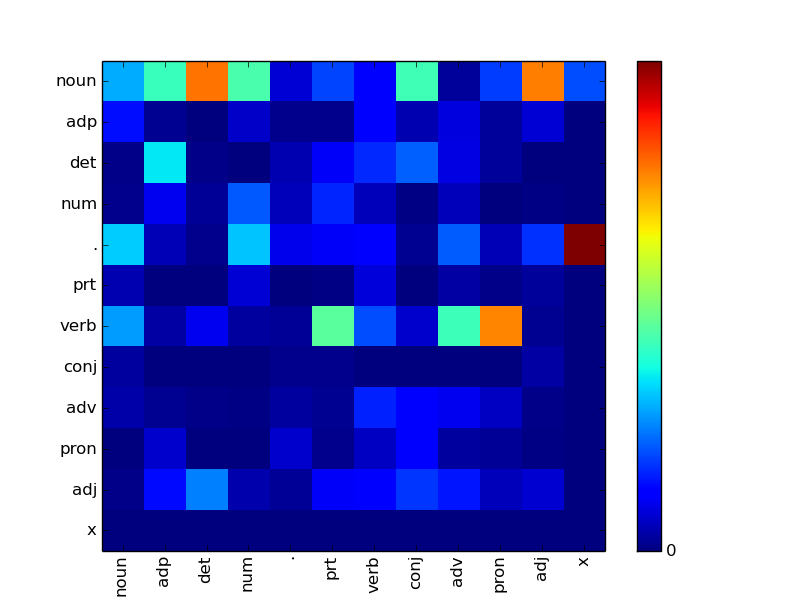
\includegraphics[scale=.5]{figs/sequences/transition_probs}
\caption{\label{fig:transProbs} Transition probabilities of the
trained model. Each column is previous state and row is current
state. Note the high probability of having Noun after Adjective, or of having Verb after Noun, as expected.}
\end{figure}

\begin{exercise}
Test the model using both posterior decoding and Viterbi decoding on
both the train and test set, using the methods in class HMM:
\begin{python}
>>> viterbi_pred_train = hmm.viterbi_decode_corpus(train_seq)
>>> posterior_pred_train = hmm.posterior_decode_corpus(train_seq)
>>> eval_viterbi_train =   hmm.evaluate_corpus(train_seq, viterbi_pred_train)
>>> eval_posterior_train =  hmm.evaluate_corpus(train_seq, posterior_pred_train)
>>> print "Train Set Accuracy: Posterior Decode \%.3f, Viterbi Decode: \%.3f"\%(eval_posterior_train,eval_viterbi_train)
Train Set Accuracy: Posterior Decode 0.985, Viterbi Decode: 0.985
>>> viterbi_pred_test = hmm.viterbi_decode_corpus(test_seq)
>>> posterior_pred_test = hmm.posterior_decode_corpus(test_seq)
>>> eval_viterbi_test =   hmm.evaluate_corpus(test_seq,viterbi_pred_test)
>>> eval_posterior_test = hmm.evaluate_corpus(test_seq,posterior_pred_test)
>>> print "Test Set Accuracy: Posterior Decode \%.3f, Viterbi Decode: \%.3f"\%(eval_posterior_test,eval_viterbi_test)
Test Set Accuracy: Posterior Decode 0.350, Viterbi Decode: 0.509
\end{python}

What do you observe? Remake the previous exercise but now train the HMM
using smoothing. Try different values (0,0.1,0.01,1) and report the results on the
train and development set. (Use function
\emph{pick\_best\_smoothing}).


\begin{python}
>>> best_smothing = hmm.pick_best_smoothing(train_seq, dev_seq, [10,1,0.1,0])
Smoothing 10.000000 --  Train Set Accuracy: Posterior Decode 0.731, Viterbi Decode: 0.691
Smoothing 10.000000 -- Test Set Accuracy: Posterior Decode 0.712, Viterbi Decode: 0.675
Smoothing 1.000000 --  Train Set Accuracy: Posterior Decode 0.887, Viterbi Decode: 0.865
Smoothing 1.000000 -- Test Set Accuracy: Posterior Decode 0.818, Viterbi Decode: 0.792
Smoothing 0.100000 --  Train Set Accuracy: Posterior Decode 0.968, Viterbi Decode: 0.965
Smoothing 0.100000 -- Test Set Accuracy: Posterior Decode 0.851, Viterbi Decode: 0.842
Smoothing 0.000000 --  Train Set Accuracy: Posterior Decode 0.985, Viterbi Decode: 0.985
Smoothing 0.000000 -- Test Set Accuracy: Posterior Decode 0.370, Viterbi Decode: 0.526
>>> hmm.train_supervised(train_seq, smoothing=best_smothing)
>>> viterbi_pred_test = hmm.viterbi_decode_corpus(test_seq)
>>> posterior_pred_test = hmm.posterior_decode_corpus(test_seq)
>>> eval_viterbi_test =   hmm.evaluate_corpus(test_seq, viterbi_pred_test)
>>> eval_posterior_test = hmm.evaluate_corpus(test_seq, posterior_pred_test)
>>> print "Best Smoothing \%f --  Test Set Accuracy: Posterior Decode \%.3f, Viterbi Decode: \%.3f"%(best_smothing,eval_posterior_test,eval_viterbi_test)
Best Smoothing 0.100000 --  Test Set Accuracy: Posterior Decode 0.837, Viterbi Decode: 0.827
\end{python}


Perform some error analysis to understand were the errors are coming
from. You can start by visualizing the confusion matrix (true tags vs
predicted tags). You should get something like \ref{fig:cm_uns}.

\begin{python}
>>> import sequences.confusion_matrix as cm
>>> confusion_matrix = cm.build_confusion_matrix(test_seq.seq_list, viterbi_pred_test, len(corpus.tag_dict), hmm.get_num_states())
>>> cm.plot_confusion_bar_graph(confusion_matrix, corpus.tag_dict, xrange(hmm.get_num_states()), 'Confusion matrix')
>>> plt.show()
\end{python}

\begin{figure}
\centering
\includegraphics[scale=.5]{figs/sequences/cm_sup.png}
\caption{\label{fig:cm_uns} Confusion Matrix for the previous
  example. Predict tags are columns and the true tags corresponds to
  the constituents of each column.}
\end{figure}

\end{exercise}


%\begin{exercise}
%Implement a function that produces the accuracy for rare words vs
%common words. Use you own definition of rare word.
%
%Can you come up with other error analysis methods? Which?
%
%\end{exercise}

%\begin{exercise}
%So far we have only worked with a limited dataset of 1000 words. Try increasing the number of sentences to 10000. What do you observe?
%\end{exercise}


%\section{Unsupervised Learning of HMMs}
%
%\afm{explain here the EM algorithm}
%
%\begin{python}
%
%Initial accuracy: 0.303638
%Iter: 1 Log Likelihood: -101824.763927
%Iter: 1 Accuracy: 0.305441
%Iter: 2 Log Likelihood: -78057.108346
%Iter: 2 Accuracy: 0.321976
%Iter: 3 Log Likelihood: -77813.725501
%Iter: 3 Accuracy: 0.357451
%Iter: 4 Log Likelihood: -77192.947674
%Iter: 4 Accuracy: 0.385109
%Iter: 5 Log Likelihood: -76191.800849
%Iter: 5 Accuracy: 0.392123
%Iter: 6 Log Likelihood: -75242.572729
%Iter: 6 Accuracy: 0.391121
%Iter: 7 Log Likelihood: -74392.892496
%Iter: 7 Accuracy: 0.404249
%Iter: 8 Log Likelihood: -73357.542833
%Iter: 8 Accuracy: 0.399940
%Iter: 9 Log Likelihood: -72135.182778
%Iter: 9 Accuracy: 0.399238
%Iter: 10 Log Likelihood: -70924.246230
%Iter: 10 Accuracy: 0.395430
%Iter: 11 Log Likelihood: -69906.561800
%Iter: 11 Accuracy: 0.394328
%Iter: 12 Log Likelihood: -69140.228623
%Iter: 12 Accuracy: 0.390821
%Iter: 13 Log Likelihood: -68541.416423
%Iter: 13 Accuracy: 0.391522
%Iter: 14 Log Likelihood: -68053.456865
%Iter: 14 Accuracy: 0.389117
%Iter: 15 Log Likelihood: -67667.318961
%Iter: 15 Accuracy: 0.386411
%Iter: 16 Log Likelihood: -67337.685686
%Iter: 16 Accuracy: 0.385409
%Iter: 17 Log Likelihood: -67054.571821
%Iter: 17 Accuracy: 0.385409
%Iter: 18 Log Likelihood: -66769.973881
%Iter: 18 Accuracy: 0.385409
%Iter: 19 Log Likelihood: -66442.608458
%Iter: 19 Accuracy: 0.385409
%
%\end{python}


\section{\label{unsupervised} Unsupervised Learning of HMMs}
We next address the problem of \emph{unsupervised} learning. 
In this setting, we are not given any labeled data; all we get to see is a set of natural language sentences.  
The underlying question is: 
\begin{quote}
Can we learn something from raw text?
\end{quote}
This task is challenging, since the process by which linguistic structures are generated is not always clear; 
and even when it is, it is typically too complex to be
formally expressed. Nevertheless, unsupervised learning has been applied to a
wide range of NLP tasks, such as: 
\pos\ Induction  \citep{schutze1995distributional,merialdo1994tet,clark03combining},
Dependency Grammar Induction \citep{klein2004acl,smith2006annealing}, Constituency Grammar Induction \citep{klein2004acl}, Statistical Word Alignments 
\citep{brown94mathematic} and Anaphora Resolution \citep{charniak2009works}, just to name a few. 

Different motivations have pushed research in this area. From both a linguistic and cognitive point of view, 
unsupervised learning is useful as a tool to study language acquisition. 
From a machine learning point of view, unsupervised learning is a fertile ground for testing new learning methods, 
where significant improvements can yet be made. 
From a more pragmatic perspective, unsupervised learning is required
since annotated corpora is a scarce resource for different reasons. Independently of the reason, unsupervised learning is an increasing active field of research.

A first problem with unsupervised learning, since we don't observe any labeled data (i.e., 
the training set is now $\mathcal{D}_{U} = \{x^1,\ldots, x^M\}$), 
is that most of the methods studied so far (e.g., Perceptron, MIRA, SVMs) cannot be used since we cannot compare 
the true output with the predicted output. 
Note also that a direct minimization of the \emph{complete negative log-likelihood} of the data, $\log P_{\theta}(X^1=x^1,\ldots,X^M=x^m)$, 
is very challenging, since it would require marginalizing out (\emph{i.e.}, summing over) all possible hidden variables:
\begin{equation}
 \log P_{\theta}(X^1=x^1,\ldots,X^M=x^m) =  \sum_{m=1}^M \log \sum_{y \in \Lambda} P_{\theta} (X=x^m,Y=y).
\end{equation}
Note also that the objective above is \emph{non-convex} even for a linear model: hence, it may have local minima, which makes optimization much 
more difficult.%
%\footnote{Another observation is that normally we are restricted to generative models, 
%with some remarkable exceptions~\citep{smith2005acl}, since the objective of discriminative models when no labels are observed are 
%meaningless ($\sum_{y^m } P(y^m |x^m) = 1$); this rules out, for instance, Maximum Entropy classifiers.}

The most common optimization method in the presence of hidden (latent) variables is the Expectation Maximization (EM) algorithm, described in the next section. Note that this algorithm is a generic optimization routine that does not depend on a particular model. Later, in Section \ref{posi} we will apply the EM algorithm to the task of part-of-speech induction, where one is given raw text and a number of clusters and the task is to cluster words that behave similarly in a grammatical sense. 

\subsection{\label{em}Expectation Maximization Algorithm}
Given the training corpus $\mathcal{D}_{U} := \{x^1, \ldots, x^M\}$, training 
seeks model parameters $\theta$ that minimize the negative log-likelihood of the corpus:
\begin{equation}
\label{loglikelihoood}
\mathbf{Negative\;Log\;Likelihood\!:}\;\;\;\; \likelihood(\theta) = \widehat{\mathbb{E}} [-\log P_{\theta}(X)] = -\frac{1}{M}\sum_{m=1}^M \log \left( \sum_{y^m \in \Lambda} P_{\theta}(X=x^m,Y=y^m) \right),
\end{equation}
where $\widehat{\mathbb{E}}[f(X)] := \frac{1}{M}\sum_{m=1}^{M} f(x^m)$ denotes the empirical average of a function $f$ over the training corpus. Because of the hidden variables $y^1,\ldots,y^M$, the likelihood term contains a
sum over all possible hidden structures inside of a logarithm, which
makes this quantity hard to compute.

The most common minimization
algorithm to fit the model parameters in the presence of hidden
variables is the Expectation-Maximization (EM) algorithm. 
The EM procedure can be thought of intuitively in the following way. 
If we observe the hidden variables' values for all sentences in the
corpus, then we could easily compute the maximum likelihood value of
the parameters as described in Section \ref{ml}. 
On the other hand, if we had the model parameters we could label data
using the model, and collect the
sufficient statistics described in Section \ref{ml}.
However, since we are working in an unsupervised setting, we never get to
observe the hidden state sequence. Instead, given the 
training set $\mathcal{D}_{U} = \{x^1 \ldots x^M\}$, we will need to
collect \emph{expected} sufficient statistics (in this case, \emph{expected} counts) 
that
represent the number of times that each hidden variable is
expected to be used with the current parameters setting. These expected sufficient
statistics will then be used during learning as ``fake'' observations of
the hidden variables. Using the node and edge posterior distributions
described in Equations \ref{eq::nodePosterior} and \ref{eq::edgePosterior},
the expected sufficient statistics can 
be computed by the following formulas:

\begin{align}
\mathbf{Initial \ Counts\!:}\;\;\;\;  &  C_{\mathrm{init}}(c_k) = \sum_{m=1}^M
P_{\theta} (Y^m_1 = c_k \,\,|\,\, X^m = x^m); \label{eq::initialCountsPost}\\
%
%\mathbf{Final \ Counts\!:}\;\;\;\;  &  fc(\hv_l,\hv _m) = \sum_{\trex} 
%\Ind (\hs_N = \hv_l \mid \hs_{N-1} = \hv_m); \label{eq::finalCounts}\\
%
\mathbf{Transition \ Counts\!:}\;\;\;\;  &  C_{\mathrm{trans}}(c_k,c_l) =
\sum_{m=1}^M  \sum_{i = 2}^{N}
P_{\theta}(Y^m_i = c_k \wedge Y^m_{i-1} = c_l \,\,|\,\, X^m = x^m); \label{eq::transitionCountsPost}\\
%
\mathbf{Final \ Counts\!:}\;\;\;\;  &  C_{\mathrm{final}}(c_k) = \sum_{m=1}^M
P_{\theta} (Y^m_N = c_k \,\,|\,\, X^m = x^m); \label{eq::finalCountsPost}\\
%
\mathbf{Emission \ Counts\!:}\;\;\;\;  &  
C_{\mathrm{emiss}}(w_j,c_k) = \sum_{m=1}^M
\sum_{i = 1}^{N}
\Ind (x^m_i = w_j) P_{\theta}(Y^m_i = c_k \,\,|\,\, X^m = x^m); \label{eq::emissionCountsPost}
\end{align}

%\begin{align}
%\mathbf{Initial \ Counts\!:}\;\;\;\;  &  ic(\hv_l) = \sum_{d=1}^D
%\gamma_1 (\hv_l); \label{eq::initialCountsPost}\\
%\mathbf{Final \ Counts\!:}\;\;\;\;  &  fc(\hv_N,\hv _{N-1}) = \sum_{d=1}^D  \xi_{N-1} (\hv_l,\hv_m); \label{eq::finalCountsPost}\\
%\mathbf{Transition \ Counts\!:}\;\;\;\;  &  tc(\hv_l,\hv _m) = \sum_{d=1}^D \sum_{i = 1}^{N-1}  \xi_i (\hv_l,\hv_m); \label{eq::transitionCountsPost}\\
%\mathbf{State \ Counts\!:}\;\;\;\;  &  sc(\vv_q,\hv_m) = \sum_{d=1}^D \sum_{i = 1 , \obs_i = \vv_q }^{N}  \gamma_i (\hv_m). \label{eq::stateCountsPost}
%\end{align}

Compare the previous equations with the ones described in Section
\ref{ml} for the same quantities (Eqs.~\ref{eq::initialCounts}--\ref{eq::emissionCounts}). The main difference is that while in
the presence of supervised data you sum the observed events, when you
have no label data you sum the posterior probabilities of each
event. If these probabilities were such that the probability mass was
around single events then both equations will produce the same result.



The EM procedure starts with an initial guess for the parameters
$\theta^0$ at time $t = 0$. The algorithm keeps iterating 
until it converges to a local minima of the negative log likelihood. Each
iteration is divided into two steps:
\begin{itemize} 
 \item The {\bf{E-Step}} (Expectation) 
computes the posteriors for the hidden variables $P_{\theta^t}(Y|X=x^m)$
given the current parameter values $\theta^t$ and the observed variables $X=x^m$ for the $m$-th sentence. 
For an HMM, this can be done through the Forward-Backward algorithm described in the previous sections.
\item The {\bf{M-step}} (Maximization) uses those posteriors $P_{\theta^t}(Y|X=x^m)$ to
``softly fill in'' the values of the hidden variables $Y^m$, and
collects the sufficient statistics: initial counts (Eq: \ref{eq::initialCountsPost}), transition counts (Eq:
\ref{eq::transitionCountsPost}), 
final counts  (Eq: \ref{eq::finalCountsPost}),
and emission counts (Eq: \ref{eq::emissionCountsPost}). These
counts are then used to estimate maximum likelihood parameters $\theta^{t+1}$, as described in
Section \ref{ml}.
\end{itemize}

The EM algorithm is guaranteed to
converge to a local minimum of the negative log-likelihood $\likelihood(\theta)$, under mild
conditions.  
Note that we are not committing to the best assignment of the hidden variables, but
summing the occurrences of each parameter weighed by the posterior
probability of all possible assignments. 
This modular split into two intuitive and straightforward steps
accounts for the vast popularity of EM.%
\footnote{More formally, EM minimizes an \emph{upper bound} of $\likelihood(\theta)$ via block-coordinate descent. See \citet{Neal1998} for details. Also, even though we are presenting EM in the context of HMMs, this algorithm can be more broadly applied to any probabilistic model with latent variables.} %

% on an upper bound $F(q,\theta)$ using an auxiliary distribution over the latent variables
%$\auxq$:
%\begin{eqnarray}
%\likelihood(\theta)  &=& \XpD \left[-\log \sum_{\hseq}\joint \right]\\
%\label{eq:jensen}&=& \XpD \left[-\log \sum_{\hseq}
%\auxq*\frac{\joint}{\auxq}\right] \le \XpD \left[- \sum_{\hseq} \auxq\log \frac{\joint}{\auxq}\right] \\
%&=& \XpD \left[\sum_{\hseq} \auxq\log \frac{\auxq}{\joint}\right] =  F(q,\theta),
%\end{eqnarray}
%where we have multiplied and divided the $\joint$ by the same quantity
%$\auxq$, and 
%the lower bound comes from applying Jensen Inequality (Equation
%\ref{eq:jensen}). $F(q,\theta)$ is normally referred to as the energy
%function, which comes from the physics field and refers to the energy of a given system that we want to minimize.
%\begin{equation}
%\mathbf{EM\;Upper\;Bound\!:}\;\;\;\;\;\likelihood(\theta) \le F(q,\theta) =
%\XpD \left[\sum_{\hseq} \auxq\log \frac{\auxq}{\joint}\right].
%\end{equation}
%The alternating E and M steps at iteration $t+1$ can be seen as minimizing the energy function first 
%with respect to $\auxq$ and then with respect to $\theta$:
%\begin{eqnarray}
%\hspace{-5mm}{\mathbf E\!:}&& q^{t+1}(\hseq\mid\sent) =
%\argmin_{\auxq} F(q,\theta^t)
%  = \argmin_{\auxq} \KL(q(\hseq\mid\sent)\,||\,p_{\theta^t}(\hseq\mid\sent)) = p_{\theta^t}(\hseq\mid\sent);
% \label{eq:e-step} \\
%\hspace{-5mm}{\mathbf M\!:}&& \theta^{t+1} = \argmin_\theta
%F(q^{t+1},\theta) = \argmax_\theta \XpD\!\left[\sum_{\hseq}
%q^{t+1}(\hseq\mid\sent)\log p_\theta(\sent,\hseq)\right];
%\label{eq:m-step}
%\end{eqnarray}
%where $\KL(q||p) = \Xp_q[\log \frac{q(\cdot)}{p(\cdot)}]$ is the
%Kullback-Leibler divergence. The KL term in the E-Step results from 
%dropping all terms from the energy function that are constant for a
%set $\theta$, in this case the likelihood of the observation sequence
%$\marginal$:
%
%\begin{align}
%\sum_{\hseq} \auxq\log \frac{\auxq}{\joint} &= \sum_{\hseq} \auxq\log
%\auxq - \sum_{\hseq} \auxq\log \joint  \\ 
%&= \sum_{\hseq} \auxq\log \auxq - \sum_{\hseq} \auxq\log \marginal
%\posterior \\
%&= \sum_{\hseq} \auxq\log \frac{\auxq}{\posterior} - \log \marginal \\
%&= \KL(\auxq||\posterior) - \log \marginal.
%\end{align}

Algorithm ~\ref{alg::em} presents the pseudo code for the EM
algorithm. 
%Note that this algorithm is agnostic of a particular model,
%it only requires the model to implement a common interface.

\begin{algorithm}
\begin{algorithmic}[1]
  \STATE {\bfseries input:} dataset $\mathcal{D}_{U}$, initial model $\theta$
    \FOR{$t = 1$ {\bfseries to} $T$}
    	  \STATE
    	  \STATE \textbf{E-Step:}
      \STATE Clear counts: $C_{\mathrm{init}}(.) = C_{\mathrm{trans}}(.,.) = C_{\mathrm{final}}(.) = C_{\mathrm{emiss}}(.,.) = 0$
      \FOR{$x^m \in \mathcal{D}_{U}$}
      	\STATE Compute posterior expectations $P_{\theta}(Y_i|X=x^m)$ and $P_{\theta}(Y_i,Y_{i+1}|X=x^m)$ using the current model $\theta$
%        \STATE posteriors,likelihood =model.compute\_posteriors($seq$)
%        \STATE model.update\_counts($seq$,posteriors)
      \STATE Update counts as shown in Eqs.~\ref{eq::initialCountsPost}--\ref{eq::emissionCountsPost}.
      \ENDFOR
    	  \STATE
      \STATE \textbf{M-Step:}
         \STATE Update the model parameters $\theta$ based on the counts.
    \ENDFOR
\end{algorithmic}    
\caption[EM algorithm]{\label{alg::em}  EM algorithm.} 
\end{algorithm}


One important thing to note in Algorithm \ref{alg::em} is that for the
HMM model we already have all the model pieces we require. In fact
the only method we don't have yet implemented from previous classes is
the method to update the counts given the posteriors. 

\begin{exercise}

Implement the method to update the counts given the state and transition posteriors.
\begin{python}
 def update_counts(self, sequence, state_posteriors, transition_posteriors):
\end{python}

%Use the method you defined previously to check the count tables to
%check if this method is correct. Use a corpus with only one sentence
%to make the test simpler.

%\begin{python}
%In []: run readers/pos_corpus.py
%In []: posc = PostagCorpus("en",max_sent_len=15,train_sents=1,dev_sents=0,test_sents=0)
%In []: run sequences/hmm.py
%In []: hmm = HMM(posc)
%In []: hmm.train_supervised(posc.train,smoothing=0.1)
%In []: hmm.clear_counts()
%In []: posteriors,likelihood = hmm.get_posteriors(posc.train.seq_list[0])
%In []: hmm.update_counts(posc.train.seq_list[0],posteriors)
%In []: hmm.sanity_check_counts(posc.train)
%\end{python}

%If you pass this test, then you have all the pieces to implement the
%EM algorithm. Look at the code for EM algorithm in file
%\emph{sequences/em.py} and check it for yourself. 

You now have all the pieces to implement the
EM algorithm. Look at the code for EM algorithm in file
\emph{sequences/hmm.py} and check it for yourself. 

\begin{python}
    def train_EM(self, dataset, smoothing=0, num_epochs=10, evaluate=True):
        self.initialize_random()

        if evaluate:
            acc = self.evaluate_EM(dataset)
            print "Initial accuracy: %f"%(acc)
            
        for t in xrange(1, num_epochs):
            #E-Step
            total_log_likelihood = 0.0
            self.clear_counts(smoothing)
            for sequence in dataset.seq_list:
                # Compute scores given the observation sequence.
                initial_scores, transition_scores, final_scores, emission_scores = \
                    self.compute_scores(sequence)
                
                state_posteriors, transition_posteriors, log_likelihood = \
                    self.compute_posteriors(initial_scores,
                                            transition_scores,
                                            final_scores,
                                            emission_scores)

                self.update_counts(sequence, state_posteriors, transition_posteriors)
                total_log_likelihood += log_likelihood
            print "Iter: %i Log Likelihood: %f"%(t, total_log_likelihood)
            #M-Step
            self.compute_parameters()
            if evaluate:
                 ### Evaluate accuracy at this iteration
                acc = self.evaluate_EM(dataset)
                print "Iter: %i Accuracy: %f"%(t,acc)
\end{python}

\end{exercise}

%%% Local Variables: 
%%% mode: latex
%%% TeX-master: "../../guide"
%%% End: 




\subsection{\label{posi}Part of Speech Induction}
In this section we present the \posi\ task. \pos\ tags are pre-requisite for many text applications. The task of \pos\ tagging where one is given a labeled training set of words and respective tags is a well studied task with several methods achieving high prediction quality, as we saw in the first part of this chapter. %Chapters \ref{day:seq} and \ref{day:seq_disc}. 

On the other hand the task of \posi\ where one does not have access to a labeled corpus is a much harder task with a huge space for improvement. In this case, we are given only the raw text along with sentence boundaries and a predefined number of clusters we can use. This problem can be seen as a clustering problem. We want to cluster words that behave grammatically in the same way on the same cluster. This is a much harder problem.

%Formally, the problem setting is the following: we are given a training set $\X = \sent^1 \ldots \sent^D$ of $D$ training examples, where each example $\sent = \obs_1 \ldots \obs_N$ is a sentence of $N$ words, whose values $\vv$ are taken from a vocabulary $\vocab$ of possible word types. We are also given the set of clusters $\hvocab$ that we are allowed to use. The hidden structure $\hseq = \hs_1 \ldots \hs_N$ corresponds to a sequence of cluster assignments for each individual word, such that $\hs_n = \hv_l$ with $\hv_l \in \hvocab$. 
%
Depending on the task at hand we can pick an arbitrary number of clusters. If the goal is to test how well our method can recover the true POS tags then we should use the same number of clusters as POS tags. On the other hand, if the task is to extract features to be used by other methods we can use a much bigger number of clusters (e.g., 200) to capture correlations not captured by POS tags, like lexical affinity. 

Note, however that nothing is said about the identity of each cluster. The model has no preference in assigning cluster 1 to nouns vs cluster 2 to nouns. Given this non-identifiability several metrics have been proposed for evaluation \citep{Reichart09,haghighi2006naacl,Meila07,RosenbergH07}. In this class we will use a common and simple metric called \textbf{1-Many}, which maps each cluster to majority pos tag that it contains (see Figure \ref{fig:cm_uns} for an example). 

\begin{figure}
\centering
\includegraphics[scale=.5]{figs/sequences/cm_uns1.png}
\caption{\label{fig:cm_uns} Confusion Matrix example. Each cluster is a column. The best tag in each column is represented under the column (1-many) mapping. Each color represents a true Pos Tag.}
\end{figure}


\begin{exercise}
Run 20 epochs of the EM algorithm for part of speech induction:
\begin{python}
>>> hmm.train_EM(train_seq, 0.1, 20, evaluate=True)
>>> viterbi_pred_test = hmm.viterbi_decode_corpus(test_seq)
>>> posterior_pred_test = hmm.posterior_decode_corpus(test_seq)
>>> eval_viterbi_test =   hmm.evaluate_corpus(test_seq, viterbi_pred_test)
>>> eval_posterior_test = hmm.evaluate_corpus(test_seq, posterior_pred_test)

Initial accuracy: 0.303638
Iter: 1 Log Likelihood: -101824.763927
Iter: 1 Accuracy: 0.305441
Iter: 2 Log Likelihood: -78057.108346
Iter: 2 Accuracy: 0.321976
Iter: 3 Log Likelihood: -77813.725501
Iter: 3 Accuracy: 0.357451
Iter: 4 Log Likelihood: -77192.947674
Iter: 4 Accuracy: 0.385109
Iter: 5 Log Likelihood: -76191.800849
Iter: 5 Accuracy: 0.392123
Iter: 6 Log Likelihood: -75242.572729
Iter: 6 Accuracy: 0.391121
Iter: 7 Log Likelihood: -74392.892496
Iter: 7 Accuracy: 0.404249
Iter: 8 Log Likelihood: -73357.542833
Iter: 8 Accuracy: 0.399940
Iter: 9 Log Likelihood: -72135.182778
Iter: 9 Accuracy: 0.399238
Iter: 10 Log Likelihood: -70924.246230
Iter: 10 Accuracy: 0.395430
Iter: 11 Log Likelihood: -69906.561800
Iter: 11 Accuracy: 0.394328
Iter: 12 Log Likelihood: -69140.228623
Iter: 12 Accuracy: 0.390821
Iter: 13 Log Likelihood: -68541.416423
Iter: 13 Accuracy: 0.391522
Iter: 14 Log Likelihood: -68053.456865
Iter: 14 Accuracy: 0.389117
Iter: 15 Log Likelihood: -67667.318961
Iter: 15 Accuracy: 0.386411
Iter: 16 Log Likelihood: -67337.685686
Iter: 16 Accuracy: 0.385409
Iter: 17 Log Likelihood: -67054.571821
Iter: 17 Accuracy: 0.385409
Iter: 18 Log Likelihood: -66769.973881
Iter: 18 Accuracy: 0.385409
Iter: 19 Log Likelihood: -66442.608458
Iter: 19 Accuracy: 0.385409

>>> confusion_matrix = cm.build_confusion_matrix(test_seq.seq_list, viterbi_pred_test, 
                                             len(corpus.tag_dict), hmm.get_num_states())
>>> cm.plot_confusion_bar_graph(confusion_matrix, corpus.tag_dict, 
                            xrange(hmm.get_num_states()), 'Confusion matrix')
\end{python}
Note: your results may not be the same as in this example since we are using a random start, but the trend should be the same, with likelihood decreasing at every iteration (\terxtbf{the values in the example are the log likelihood, or the negative log likelihhod? if it is the fisrt, it is actually increasing}). 
%Also note that in some iterations the likelihood does not go down because of some rounding errors, however the general trend is that likelihood decreases over iterations. 
\end{exercise}

In the previous exercise we used an HMM to do Part-of-Speech induction using 12 clusters (by omission the HMM uses as number of hidden states the one provided by the corpus). A first observation is that the log-likelihood is always increasing as expected. Another observation is that the accuracy goes up from 33\% to 41\%. Note that normally you will run this algorithm for 200 iterations, we stopped earlier for time constraints. Another observations is that the accuracy is not monotonic increasing, this is because the likelihood is not a perfect proxy for the accuracy. In fact all that likelihood is measuring are co-occurrences of words in the corpus; it has no idea of pos tags. The fact we are improving derives from the fact that language is not random but follows some specific hidden patterns. In fact this patterns are what true pos-tags try to capture. A final observation is that the performance is really bad compared to the supervised scenario, so there is a lot of space for improvement. The actual state of the art is around 71\% for fully unsupervised~\citep{JoaoThesis,bergkirkpatrick2010naacl} and 80\% \citep{das-petrov:2011:ACL-HLT2011} using parallel data and information from labels in the other language. 

Looking at Figure \ref{fig:cm_uns} shows the confusion matrix for this particular example. 
A first observation is that most clusters are mapped to nouns, verbs or punctuation. 
This is a known fact since there are many more nouns and verbs than any other tags. Since maximum likelihood prefers probabilities 
to be uniform (imagine two parameters: in one setting both have value 0.5 so the likelihood will be 0.5*0.5 = 0.25, 
while in the other case one as 0.1 and 0.9 so the maximum likelihood is 0.09). Several approaches have been proposed to 
address this problem, moving towards a Bayesian setting \citep{johnson2007dtf}, or using 
Posterior Regularization \citep{graca2009nips}. 
%more about this later today. 
%Part-of-Speech induction is a very active field of research, in fact in the last two ACL conferences (Association for Computational Linguistics) the short paper award (2010) and the best paper award (2011) were about this topic~\citep{lamar-EtAl:2010:Short,das-petrov:2011:ACL-HLT2011}.








% \begin{exercise}

% Repeat the previous exercise using a different number of hidden states (20,50). Note that the higher the number of states is the slower the training will be.
% What do you observe? Look at the confusion matrix and try to explaing what is happening.

% \begin{python}
% In []: run readers/pos_corpus.py
% In []: posc = PostagCorpus("en",max_sent_len=15,train_sents=1000,dev_sents=0,test_sents=0)
% In []: run sequences/hmm.py
% In []: hmm = HMM(posc,nr_states=20)
% In []: hmm.initialize_radom()
% In []: run sequences/em.py
% In []: em = EM(posc,hmm)
% In []: em.train(posc.train,nr_iter=20)
% Init acc 0.348933
% Iter: 1 Negative Log Likelihood 16.038424
% Iter: 1 acc 0.362662
% Iter: 2 Negative Log Likelihood 11.200816
% Iter: 2 acc 0.370177
% Iter: 3 Negative Log Likelihood 11.046597
% Iter: 3 acc 0.380800
% Iter: 4 Negative Log Likelihood 10.607496
% Iter: 4 acc 0.389518
% Iter: 5 Negative Log Likelihood 9.809817
% Iter: 5 acc 0.394027
% Iter: 6 Negative Log Likelihood 8.949717
% Iter: 6 acc 0.396733
% Iter: 7 Negative Log Likelihood 8.105404
% Iter: 7 acc 0.398337
% Iter: 8 Negative Log Likelihood 7.366612
% Iter: 8 acc 0.392925
% Iter: 9 Negative Log Likelihood 7.005009
% Iter: 9 acc 0.393126
% Iter: 10 Negative Log Likelihood 6.895723
% Iter: 10 acc 0.397034
% Iter: 11 Negative Log Likelihood 6.851836
% Iter: 11 acc 0.397134
% Iter: 12 Negative Log Likelihood 6.818365
% Iter: 12 acc 0.399238
% Iter: 13 Negative Log Likelihood 6.782213
% Iter: 13 acc 0.406053
% Iter: 14 Negative Log Likelihood 6.755121
% Iter: 15 Negative Log Likelihood 6.745873
% Iter: 15 acc 0.419681
% Iter: 16 Negative Log Likelihood 6.743681
% Iter: 16 acc 0.424291
% Iter: 17 Negative Log Likelihood 6.745030
% Iter: 17 acc 0.431406
% Iter: 18 Negative Log Likelihood 6.747628
% Iter: 18 acc 0.434512
% Iter: 19 Negative Log Likelihood 6.749084
% Iter: 19 acc 0.438721
% pred = hmm.viterbi_decode_corpus(posc.train.seq_list)
% cm = build_confusion_matrix(posc.train.seq_list,pred,len(posc.int_to_pos),hmm.nr_states)
% plot_confusion_bar_graph(cm,posc.int_to_pos,range(12),"test")
% \end{python}

% \end{exercise}

%%% Local Variables: 
%%% mode: latex
%%% TeX-master: "../../guide"
%%% End: 




%%% Local Variables: 
%%% mode: latex
%%% TeX-master: "../../guide"
%%% End: 





%\section{\label{hmm_special_state} HMM Initial and Final State}
%\input{pages/sequences/init_final_hmm.tex}

%\section{\label{hmm} Second order HMM}
%\input{pages/sequences/second_order_hmm.tex}


%%% Local Variables: 
%%% mode: latex
%%% TeX-master: "../../guide.tex"
%%% End: 
